\documentclass[article, onecolumn]{IEEEtran}

\usepackage{cite}
\ifCLASSINFOpdf
	\usepackage[pdftex]{graphicx}
	\graphicspath{{./tikz_figures/}}
	\DeclareGraphicsExtensions{.pdf,.jpeg,.png, .jpg, .PNG}
\else
\fi
\usepackage{amsmath,bm}
\interdisplaylinepenalty=2500
\ifCLASSOPTIONcompsoc
	\usepackage[caption=false,font=normalsize,labelfont=sf,textfont=sf]{subfig}
\else
	\usepackage[caption=false,font=footnotesize]{subfig}
\fi
\usepackage{url}
\usepackage{amsfonts} % for \mathbb{}
\usepackage{listings} % For writing math in verbatim
\usepackage{enumerate}

\usepackage[showlabels,sections,floats,textmath,displaymath]{preview}
\usepackage{amssymb} %% For showing special symbols like \bigstar
\usepackage{pifont}  %% For showing circled numbers
\usepackage{array}
\usepackage{algorithm}
\usepackage{algpseudocode}
\usepackage{ifthen}
\usepackage{dirtree}
\setlength{\DTbaselineskip}{13pt}
\renewcommand*\DTstyle{}
\DTsetlength{.2em}{1em}{.2em}{.4pt}{2pt}

\newcommand{\mathnew}{\mathit} 
% for nice reference 
\newcommand{\fsp}{{\;}}
\newcommand{\Fig}{\figurename \fsp}
\newcommand{\Sec}{Sec.\fsp}
\newcommand{\Eq}{Eq.\fsp}
\newcommand{\Tab}{Tab.\fsp}
\newcommand{\Alg}{Alg.\fsp}
\newcommand{\etal}{\textit{et al}. }
\newcommand{\ie}{\textit{i}.\textit{e}. }
\newcommand{\eg}{\textit{e}.\textit{g}. }
\newcommand{\Prop}{Property }

\DeclareMathOperator*{\argminB}{argmin} 

\hyphenation{temperature} % correct bad hyphenation here

\usepackage{tikz}
\usetikzlibrary{arrows}
\usetikzlibrary{intersections}
\usetikzlibrary{calc, quotes}
\usetikzlibrary{external}
\tikzexternalize[prefix=tikz_figures/]%
\pgfdeclarelayer{bg}    % declare background layer
\pgfsetlayers{bg,main} % set the order of the layers (main is the standard layer)
\usetikzlibrary{patterns}
\usetikzlibrary{decorations.pathreplacing,calligraphy}

\renewcommand\thesection{\arabic{section}}
\renewcommand\thesubsectiondis{\textbf{\thesection.\arabic{subsection}}} %% This is to change the looking of subsection heading number
\renewcommand\thesubsection{\thesection.\arabic{subsection}} %% This is to change the numbering by \ref{}
\renewcommand\thesubsubsectiondis{\ding{42}\;\thesection.\arabic{subsection}.\arabic{subsubsection}}

\setcounter{tocdepth}{1} % Show sections
%\setcounter{tocdepth}{2} % + subsections
%\setcounter{tocdepth}{3} % + subsubsections
%\setcounter{tocdepth}{4} % + paragraphs
%\setcounter{tocdepth}{5} % + subparagraphs

%% The following commands are used to reduce the space before and after formula
%% in align and equation environments
%\setlength{\abovedisplayskip}{1pt}
%\setlength{\belowdisplayskip}{0pt}
%\setlength{\abovedisplayshortskip}{0pt}
%\setlength{\belowdisplayshortskip}{0pt}

%%
%% The following definition is a remedy of the fact that
%% IEEEtrans class does not define subparagraph.
%% Check this post for details
%% https://tex.stackexchange.com/a/8362/172530
\newcommand{\subparagraph}{}
\usepackage{titlesec} % for controlling vertical space around section headers
\titlespacing\section{0pt}{8pt plus 2pt minus 2pt}{4pt plus 2pt minus 2pt}
\titlespacing\subsection{0pt}{6pt plus 2pt minus 2pt}{2pt plus 2pt minus 2pt}
\titlespacing\subsubsection{0pt}{4pt plus 2pt minus 2pt}{2pt plus 1pt minus 1pt}

\titleformat{\subsection}
{\normalfont\bfseries}
{\thesubsection}{1em}{}

%%
%% Check this post for how to write properly-sized ceiling operator
%% https://tex.stackexchange.com/a/367035/172530
%%
\usepackage{mathtools}
\DeclarePairedDelimiter{\ceil}{\lceil}{\rceil}
\DeclarePairedDelimiter{\floor}{\lfloor}{\rfloor}

%% For text color
\usepackage{xcolor}

%% For drawing boxes around text
%% https://tex.stackexchange.com/a/234195/172530
\newcommand\textbox[2]{%
  \tikz[baseline]\node[%
  inner ysep=0pt, 
  inner xsep=2pt, 
  anchor=text, 
  rectangle, 
  rounded corners=1mm,
  #1] {\strut#2};%
}

%% package for highlighting text
%% Usage: \hl{text to be highlighted}
\usepackage{soul}
\sethlcolor{yellow}

%% underlining for emphasis
%% Examples:
%% \uline{important} underline
%% \uuline{urgent} double-underline
%% \uwave{boat} wavy underline like
%% \sout{wrong} line struck through word
%% \xout{removed} removed
%% \dashuline{dashing} dashed
%% \dotuline{dotty} dotted
\usepackage[normalem]{ulem}

%% define a red check mark
\newcommand\redcheck{
  {\textcolor{red}{\ding{52}}}
}

\usepackage{dblfloatfix}    % To enable figures at the bottom of page

\usepackage{wrapfig}
\usepackage{siunitx}

% Overlay question mark on equal mark
\def\qeq{\mathrel{%
    \mathchoice{\QEQ}{\QEQ}{\scriptsize\QEQ}{\tiny\QEQ}%
}}
\def\QEQ{{%
    \setbox0\hbox{=}%
    \rlap{\hbox to \wd0{\hss?\hss}}\box0
  }}

%% Package for theorem-like blocks
\usepackage{amsthm}
\renewcommand\qedsymbol{$\blacksquare$}
\newtheorem{prop}{Property}

%%%%%%%%%%%%%%%%%%%%%%%%%%%%%%%%%%%%%%%%%%%%%%%%%%%%%%%%%%
%% Tikz figure commands
%%%%%%%%%%%%%%%%%%%%%%%%%%%%%%%%%%%%%%%%%%%%%%%%%%%%%%%%%%
\newcommand{\defs}[1]{
  %% #1: gap
  \def\latalu{6}
  \def\latmem{24}
  \def\unit{.1}
  \def\h{.2}
  \def\scale{.7}
  \def\alpha{6}
  \def\numwarps{6}
  \def\gap{#1}
  \pgfmathsetmacro\latwarp{\alpha*\latalu*\unit+\latmem*\unit+\alpha*\gap*\unit-\gap*\unit}
  \pgfmathsetmacro\span{\alpha*\latalu+\latmem+\alpha*\gap-\gap+\numwarps-1}
}

\newcommand{\cycles}[2]{
  %% #1: height of the line
  %% #2: number of cycles
  \foreach \i in {0,...,#2}
  {
    \draw [ultra thin, red] ($(TL)+(\i*.1, 0)$) -- ++(0, -#1);
  }
}

\newcommand{\mylabel}[4]{
  %% #1 width of the label
  %% #2 text for the label
  %% #3 scale
  %% #4 below of above
  %% The left is defined as the coordinate before calling this command
  \coordinate (right) at ($(left)+(#1, 0)$);
  \node [scale=#3, #4, inner xsep=0] (label) at ($(left)!.5!(right)$) {#2};
  \draw [ultra thin] (left) |- (label.west); 
  \draw [ultra thin] (right) |- (label.east); 
}

\newcommand{\latlabel}[1]{
  %% #1: scale of the text
  %% (left) should be defined as the topleft of the warp
  \mylabel{\latalu*\unit}{$\text{lat}_\text{alu}$}{\scale}{above};
  \coordinate (left) at ($(left)+(\alpha*\latalu*\unit+\alpha*\gap*\unit-\gap*\unit, 0)$);
  \mylabel{\latmem*\unit}{$\text{lat}_\text{mem}$}{\scale}{above};
}

\newcommand{\coord}[3]{
  %% origin is defined as a coordinate
  %% #1: x length
  %% #2: y length
  %% #3: scale
  \draw [fill=black] (origin) circle (2pt);
  \draw [thick, ->, >=stealth, name path=x] (origin) -- ++(#1, 0)
  node [scale=#3, right] {$n$};
  \draw [thick, ->, >=stealth, name path=y] (origin) -- ++(0, #2)
  node [scale=#3, above] {$\text{thr}_\text{warp}$};  
}
\newcommand{\maxthralu}[4]{
  %% #1: \alpha, i.e. number of alu insts per warp
  %% #2: number of warps 
  %% #3: starting index of the first warp in this group
  %% #4: gap between consecutive alu insts
  %% (TL) should already be defined
  \pgfmathsetmacro\alp{int(#1-1)}
  \pgfmathsetmacro\warps{int(#2-1)}
  \foreach \w in {0,...,\warps} {
    \pgfmathsetmacro\z{int(#3+\w)}
    \node [left, scale=.9*\scale] at ($(TL)+(\w*\unit,-\w*\h-.5*\h)$) {w\z};
    \foreach \i in {0,...,\alp} {
      \draw [thick] ($(TL)+(\i*#4*\unit+\i*\latalu*\unit+\w*\unit, -\w*\h)$)
      rectangle ++(\latalu*\unit, -\h);
    }
  }
}

\newcommand{\maxthrmem}[1]{
  %% #1: number of warps 
  %% (memTL) should already be defined
  \pgfmathsetmacro\warps{int(#1-1)}
  \foreach \w in {0,...,\warps} {
    \draw [thick, blue] ($(memTL)+(\w*\unit, -\w*\h)$)
    rectangle ++(\latmem*\unit, -\h);
  }
}

\newcommand{\drawwarp}[4]{
  %% parameters same as \maxthralu
  %% #1: \alpha, i.e. number of alu insts per warp
  %% #2: number of warps 
  %% #3: starting index of the first warp in this group
  %% #4: gap between consecutive alu insts
  %% (TL) should already be defined
  \maxthralu{#1}{#2}{#3}{#4};
  \coordinate (memTL) at ($(TL)+(#1*\latalu*\unit+#1*#4*\unit-#4*\unit, 0)$);
  \maxthrmem{#2};
}

\newcommand{\myPerfModel}[1]{
  %% #1 scale
  
  % \draw [help lines] (-4,3) grid (4, -3);
  % \draw (0,0) circle (2pt);

  \def\scale{#1}

  %% Draw latency mode
  \coordinate (origin) at (-3,0);
  \coord{5}{3}{\scale};
  \coordinate (P) at ($(origin)+(1.5,1.5)$);
  \draw [ultra thick] (origin)
  --node [midway, above, sloped, align=center, scale=.8*\scale] {latency mode} (P);
  \draw [ultra thin, densely dashed] (P) -- (P |- origin)
  node [below, scale=\scale] {$n_\text{lat}$};
  \draw [ultra thin, densely dashed] (P) -- (P -| origin)
  node [left, scale=\scale] {$\text{thr}_\text{lat}$};
  %% Draw gradual saturate effect
  \coordinate (Q) at ($(P)+(1,.5)$);
  \draw [ultra thick] (P) to[out=40, in=185]
  node [scale=.7*\scale, midway, align=center, below, yshift=-1ex, xshift=1.5ex]
  {gradual\\saturate\\effect} (Q);
  \draw [ultra thin, densely dashed] (Q) -- (Q |- origin)
  node [below, scale=\scale] {$n_\text{thr}$};
  \draw [ultra thin, densely dashed] (Q) -- (Q -| origin)
  node [left, scale=\scale] {$\text{maxThr}_\text{warp}$};
  %% Draw throughput mode
  \draw [ultra thick] (Q) --node [midway, above, sloped, align=center, scale=.8*\scale]
  {Throughput mode} ++(2, 0);
}

\newcommand{\volkovPerfModel}[1]{
  %% #1 scale
  
  % \draw [help lines] (-4,3) grid (4, -3);
  % \draw (0,0) circle (2pt);

  \def\scale{#1}

  %% Draw latency mode
  \coordinate (origin) at (-3,0);
  \coord{5}{3}{\scale};
  \coordinate (P) at ($(origin)+(2,2)$);
  \draw [ultra thick] (origin)
  --node [midway, above, sloped, align=center, scale=.9*\scale] {latency mode} (P);
  \draw [ultra thin, densely dashed] (P) -- (P |- origin)
  node [below, scale=\scale] {$n_\text{tran}$};
  \draw [ultra thin, densely dashed] (P) -- (P -| origin)
  node [left, scale=\scale] {$\text{maxThr}_\text{warp}$};
  %% Draw gradual saturate effect
  % \coordinate (Q) at ($(P)+(1,.5)$);
  % \draw [ultra thick] (P) to[out=40, in=185]
  % node [scale=.7*\scale, midway, align=center, below, yshift=-1ex, xshift=1.5ex]
  % {gradual\\saturate\\effect} (Q);
  % \draw [ultra thin, densely dashed] (Q) -- (Q |- origin)
  % node [below, scale=\scale] {$n_\text{thr}$};
  % \draw [ultra thin, densely dashed] (Q) -- (Q -| origin)
  % node [left, scale=\scale] {$\text{maxThr}_\text{warp}$};
  %% Draw throughput mode
  \draw [ultra thick] (P) --node [midway, above, sloped, align=center, scale=.9*\scale]
  {Throughput mode} ++(2.5, 0);
}

\newcommand{\demoLittle}{
  \draw [help lines] (-4,3) grid (4, -3);
  \draw (0,0) circle (2pt);

  \defs{0}
  \pgfmathsetmacro\span{\alpha*\latalu+\latmem+\alpha*\gap-\gap}
  \pgfmathsetmacro\cycleh{\numwarps*\h}

  \coordinate (TL) at (-4, 3);
  \coordinate (origin) at (TL);

  \cycles{\cycleh}{\span}
  \coordinate (warp0TL) at (TL);
  \drawwarp{\alpha}{1}{0}{\gap};

  %% Draw label
  \coordinate (left) at (TL);
  \latlabel{\scale}
  
  %% 1-5 warps
  \foreach \row in {1,...,5}
  {
    %% Every line draws two warps
    %% right: (TL) = ($(TL)+(5*\unit, -\h*\row)$)
    %% left: (TL) = ($(TL)$+(-\latwarp, 0))
    %% Right warp
    \pgfmathsetmacro\lidx{int(2*\row-1)}
    \pgfmathsetmacro\ridx{int(2*\row)}
    \coordinate (TL) at ($(TL)+(5*\unit,-\h)$);
    \coordinate (oldTL) at (TL);
    \drawwarp{\alpha}{1}{\ridx}{\gap};
    %% Left warp
    \coordinate (TL) at ($(TL)+(-\latwarp, 0)$);
    \drawwarp{\alpha}{1}{\lidx}{\gap};
    \coordinate (TL) at (oldTL);
  }

  %% Draw period Dealt T
  \coordinate (left) at ($(origin)+(0,-\numwarps*\h)$);
  \mylabel{\latwarp}{$\Delta T$}{\scale}{below};
  \coordinate (left) at ($(origin)+(3*\latalu*\unit+5*\unit,0)$);
  \mylabel{2*\latalu*\unit}{$\Delta T'$}{\scale}{above};
}

\newcommand{\labelCycle}[1]{
  %% #1: cycle number
  %% (TL) should be defined
  %% \numwarps should be defined
  \coordinate (p) at ($(TL)+(#1*\unit, -\numwarps*\h)$);
  \node [scale=\scale, below left, inner sep=0] (pNode) at ($(p)+(-.2,-.2)$) {cycle #1};
  \draw [->, >=stealth] (pNode.north east) -- (p)
}

\newcommand{\labelCycleRight}[1]{
  %% #1: cycle number
  %% (TL) should be defined
  %% \numwarps should be defined
  \coordinate (p) at ($(TL)+(#1*\unit, -\numwarps*\h)$);
  \node [scale=\scale, below right, inner sep=0] (pNode) at ($(p)+(.2,-.2)$) {cycle #1};
  \draw [->, >=stealth] (pNode.north west) -- (p)
}

\newcommand{\labelCycleAbove}[1]{
  %% #1: cycle number
  %% (TL) should be defined
  %% \numwarps should be defined
  \coordinate (p) at ($(TL)+(#1*\unit, 0)$);
  \node [scale=\scale, above left, inner sep=0, align=center] (pNode) at ($(p)+(-.2,.2)$) {cycle #1};
  \draw [->, >=stealth] (pNode.south east) -- (p)
}

\newcommand{\labelCycleAboveRight}[1]{
  %% #1: cycle number
  %% (TL) should be defined
  %% \numwarps should be defined
  \coordinate (p) at ($(TL)+(#1*\unit, 0)$);
  \node [scale=\scale, above right, inner sep=0, align=center] (pNode) at ($(p)+(.2,.2)$) {cycle #1};
  \draw [->, >=stealth] (pNode.south west) -- (p)
}

\newcommand{\demoGap}{
  %% #1: scale
  \defs{0}
  \def\scale{.7}
  \coordinate (TL) at (-4, 3);
  \coordinate (origin) at (TL);
  \cycles{1.2}{\span}

  \def\gap{0}
  \drawwarp{\alpha}{\numwarps}{0}{\gap};

  %% Draw label
  \coordinate (left) at (origin);
  \latlabel{\scale}

  %% Draw arrows
  \def\arrowl{3*\latalu*\unit}
  \coordinate (ArrowL) at ($(origin)+(\latwarp+\numwarps*\unit+.4, -\numwarps/2*\h)$);
  \draw [->, >=stealth, thick] (ArrowL) --
  node[above, midway,scale=\scale] {Add 1 warp} ++(\arrowl,0);

  \coordinate (TL) at ($(origin)+(\latwarp+\numwarps*\unit+.4+\arrowl+.4,0)$);
  \def\gap{1}
  \def\numwarps{7}
  \pgfmathsetmacro\span{\alpha*\latalu+\latmem+\alpha*\gap-\gap+\numwarps-1}
  \cycles{1.4}{\span}
  \drawwarp{\alpha}{7}{0}{\gap};
   %% Draw label
  \coordinate (left) at (TL);
  \latlabel{\scale}
  %% Draw label for gap
  \node [below, scale=\scale] (gapNode) at ($(TL)+(3*\latalu*\unit+8.5*\unit,-7*\h-.2)$)
  {gaps};
  \coordinate (gap) at ($(TL)+(\latalu*\unit+6.5*\unit,-7*\h)$);
  \foreach \g in {0,1,2,3,4} {
    \draw [->, >=stealth] (gapNode.north) -| ($(gap)+(\g*\latalu*\unit+\g*\unit,0)$);
  }
  \labelCycle{6};
  %% Draw the victim alu inst
  \draw [thick, fill=gray] ($(TL)+(\latalu*\unit+\gap*\unit,0)$) rectangle ++(\latalu*\unit, -\h);
}

\newcommand{\demoSmartSched}{
  %% #1: scale
  \defs{0}
  \def\alpha{4}
  \def\latalu{4}
  \def\numwarps{4}
  \def\latmem{32}

  \pgfmathsetmacro\latwarp{\alpha*\latalu*\unit+\latmem*\unit+\alpha*\gap*\unit-\gap*\unit}
  \pgfmathsetmacro\span{\alpha*\latalu+\latmem+\alpha*\gap-\gap+\numwarps-1}
  \pgfmathsetmacro\height{\numwarps*\h}
  
  \def\scale{.7}

  %% Draw the old state of the system
  \coordinate (TL) at (-4, 3);
  \coordinate (origin) at (TL);
  \cycles{\height}{\span}
  \def\gap{0}
  \drawwarp{\alpha}{\numwarps}{0}{\gap};
  \coordinate (left) at (TL);
  \mylabel{\latwarp}{$\Delta T$}{\scale}{above};
  \coordinate (left) at ($(TL)+(0,-\numwarps*\h)$);
  \mylabel{.5*\latwarp}{$\Delta T_1$}{\scale}{below};
  \coordinate (left) at ($(TL)+(.5*\latwarp,-\numwarps*\h)$);
  \mylabel{.5*\latwarp}{$\Delta T_2$}{\scale}{below};

  %% Draw arrows
  \def\arrowl{5*\latalu*\unit}
  \coordinate (ArrowL) at ($(origin)+(\latwarp+\numwarps*\unit+.4, -\numwarps/2*\h)$);
  \draw [->, >=stealth, thick] (ArrowL) --
  node[above, midway,scale=\scale] {Add more warps} ++(\arrowl,0);

  %% Draw the new state of the system 
  \coordinate (TL) at ($(origin)+(\latwarp+\numwarps*\unit+.4+\arrowl+.4,0)$);
  \coordinate (origin) at (TL);
  \pgfmathsetmacro\height{\numwarps*\h}
  \cycles{\height}{\span}
  \drawwarp{\alpha}{\numwarps}{0}{\gap};

  \coordinate (TL) at ($(TL)+(\alpha*\latalu*\unit,-\numwarps*\h)$);
  \cycles{\height}{\span}
  \drawwarp{\alpha}{\numwarps}{4}{\gap};

  \coordinate (TL) at ($(TL)+(\alpha*\latalu*\unit,-\numwarps*\h)$);
  \pgfmathsetmacro\span{\alpha*\latalu+\latmem+\alpha*\gap-\gap}
  \cycles{\h}{\span}
  \drawwarp{\alpha}{1}{8}{\gap};

  \def\numwarps{9}
  \coordinate (left) at ($(origin)+(0, -\numwarps*\h)$);
  \mylabel{.5*\latwarp}{$\Delta T_1$}{\scale}{below};
  \coordinate (left) at ($(origin)+(\latwarp*.5, -\numwarps*\h)$);
  \mylabel{\latwarp*.5}{$\Delta T_2$}{\scale}{below};

  %% label some cycles
  \def\numwarps{9}
  \coordinate (TL) at (origin);
  \labelCycleAbove{48};
  \labelCycleAbove{16};
  \labelCycleAbove{4};
  \labelCycleAbove{33};
}

\newcommand{\demoPerfectSched}{
  %% #1: scale
  \defs{0}
  \def\alpha{4}
  \def\latalu{4}
  \def\numwarps{4}
  \def\latmem{35}

  \pgfmathsetmacro\latwarp{\alpha*\latalu*\unit+\latmem*\unit+\alpha*\gap*\unit-\gap*\unit}
  \pgfmathsetmacro\span{\alpha*\latalu+\latmem+\alpha*\gap-\gap+\numwarps-1}
  \pgfmathsetmacro\height{\numwarps*\h}
  
  \def\scale{.7}

  %% Draw the old state of the system
  \coordinate (TL) at (-4, 3);
  \coordinate (origin) at (TL);
  % \cycles{\height}{\span}
  % \def\gap{0}
  % \drawwarp{\alpha}{\numwarps}{0}{\gap};
  % \coordinate (left) at (TL);
  % \mylabel{\latwarp}{$\Delta T$}{\scale}{above};
  % \coordinate (left) at ($(TL)+(0,-\numwarps*\h)$);
  % \mylabel{.5*\latwarp}{$\Delta T_1$}{\scale}{below};
  % \coordinate (left) at ($(TL)+(.5*\latwarp,-\numwarps*\h)$);
  % \mylabel{.5*\latwarp}{$\Delta T_2$}{\scale}{below};

  % %% Draw arrows
  % \def\arrowl{5*\latalu*\unit}
  % \coordinate (ArrowL) at ($(origin)+(\latwarp+\numwarps*\unit+.4, -\numwarps/2*\h)$);
  % \draw [->, >=stealth, thick] (ArrowL) --
  % node[above, midway,scale=\scale] {Add more warps} ++(\arrowl,0);

  %% Draw the new state of the system 
  %\coordinate (TL) at ($(origin)+(\latwarp+\numwarps*\unit+.4+\arrowl+.4,0)$);
  %\coordinate (origin) at (TL);
  \pgfmathsetmacro\height{\numwarps*\h}
  \cycles{\height}{\span}
  \drawwarp{\alpha}{\numwarps}{0}{\gap};

  \coordinate (TL) at ($(TL)+(\alpha*\latalu*\unit,-\numwarps*\h)$);
  \cycles{\height}{\span}
  \drawwarp{\alpha}{\numwarps}{4}{\gap};

  \coordinate (TL) at ($(TL)+(\alpha*\latalu*\unit,-\numwarps*\h)$);
  %\pgfmathsetmacro\span{\alpha*\latalu+\latmem+\alpha*\gap-\gap}
  \cycles{\height}{\span}
  \drawwarp{\alpha}{\numwarps}{8}{\gap};

  % \def\numwarps{9}
  % \coordinate (left) at ($(origin)+(0, -\numwarps*\h)$);
  % \mylabel{.5*\latwarp}{$\Delta T_1$}{\scale}{below};
  % \coordinate (left) at ($(origin)+(\latwarp*.5, -\numwarps*\h)$);
  % \mylabel{\latwarp*.5}{$\Delta T_2$}{\scale}{below};

  %% label some cycles
  \def\numwarps{12}
  \coordinate (TL) at (origin);
  \labelCycle{48};
  \labelCycleAbove{16};
  \labelCycleAbove{4};
  \labelCycleRight{51};
}


\newcommand{\demoGapNew}{
  %% #1: scale
  \defs{0}
  \def\scale{.7}
  \coordinate (TL) at (-4, 3);
  \coordinate (origin) at (TL);
  \cycles{1.2}{\span}

  %\def\gap{0}
  %\drawwarp{\alpha}{\numwarps}{0}{\gap};

  

  \def\gap{24}
  \def\numwarps{30}
  \pgfmathsetmacro\span{\alpha*\latalu+\latmem+\alpha*\gap-\gap+\numwarps-1}
  \cycles{1.4}{\span}
  \drawwarp{\alpha}{\numwarps}{0}{\gap};
   %% Draw label
  %\coordinate (left) at (TL);
  %\latlabel{\scale}
  %% Draw label for gap
  
}

\newcommand{\tensor}[4]{
  %% (TL): predefined points of the TL corner of the tensor
  %% #1: height
  %% #2: width
  %% #3: channel
  %% #4: unit
  \def\unit{#4}
  \def\h{#1}
  \def\w{#2}
  \def\c{#3}
  \pgfmathsetmacro\halfunit{0.5*\unit}
  \pgfmathsetmacro\smallunit{0.3*\unit}

  % \draw (TL) rectangle ++(\w*\unit, -\h*\unit);
  %% horizontal lines
  \foreach \i in {0,...,\h}{
    \draw ($(TL)+(0,-\i*\unit)$) -- ++(\w*\unit,0);
  }
  \foreach \i in {1,...,\c}{
    \draw ($(TL)+(\i*\halfunit,\i*\smallunit)$) -- ++(\w*\unit,0);
  }
  %% vertical lines
  \foreach \i in {0,...,\w}{
    \draw ($(TL)+(\i*\unit,0)$) -- ++(0, -\h*\unit);
  }
  \foreach \i in {1,...,\c}{
    \draw ($(TL)+(\w*\unit+\i*\halfunit,\i*\smallunit)$) -- ++(0, -\h*\unit);
  }
  %% inclined lines
  \foreach \i in {0,...,\w}{
    \draw ($(TL)+(\i*\unit,0)$) -- ++(\c*\halfunit, \c*\smallunit);
  }
  \foreach \i in {1,...,\h}{
    \draw ($(TL)+(\w*\unit,-\i*\unit)$) -- ++(\c*\halfunit,\c*\smallunit);
  }

  %% define some anchor points
  \coordinate (backTL) at ($(TL)+(\c*\halfunit, \c*\smallunit)$);
  \coordinate (backTR) at ($(TL)+(\c*\halfunit+\w*\unit, \c*\smallunit)$);
}


\newcommand{\fillTopParallelogram}[4]{
  %% (BL) predefined point
  %% #1: height
  %% #2: width
  %% #3: shift
  %% #4: color
  \def\h{#1}
  \def\w{#2}
  \def\shift{#3}
  \def\color{#4}
  \draw [fill=\color] (BL) -- ++(\w,0) -- ++(\shift, \h)
  -- ++(-\w, 0) -- ++(-\shift, -\h);
}

\newcommand{\fillSideParallelogram}[4]{
  %% (BL) predefined point
  %% #1: height
  %% #2: width
  %% #3: shift
  %% #4: color
  \def\h{#1}
  \def\w{#2}
  \def\shift{#3}
  \def\color{#4}
  \draw [fill=\color] (BL) -- ++(\w,\shift) -- ++(0, \h)
  -- ++(-\w, -\shift) -- ++(0, -\h);
}

\newcommand{\fillRec}[3]{
  %% (TL) predefined point
  %% #1: height
  %% #2: width
  %% #3: color
  \def\h{#1}
  \def\w{#2}
  \def\color{#3}
  \draw [fill=\color] (TL) rectangle ++(\w, -\h);
}

\newcommand{\colorTensorFront}[4]{
  %% (TL): predefined points of the TL corner of the tensor
  %% #1: height
  %% #2: width
  %% #3: unit
  %% #4: color
  \def\h{#1}
  \def\w{#2}
  \def\unit{#3}
  \def\basecolor{#4}

  \coordinate (orig) at (TL);
  \coordinate (colorTensorFrontreturn) at (TL);
  %% Color the front pixels
  \foreach \row in {1,...,\h}{
    \foreach \col in {1,...,\w}{
      \coordinate (TL) at ($(orig)+(\col*\unit-\unit, -\row*\unit+\unit)$);
      \fillRec{\unit}{\unit}{\basecolor}
    }
  }

  %% restore TL
  \coordinate (TL) at (colorTensorFrontreturn);
}

\newcommand{\colorTensorTopAndSide}[6]{
  %% (TL): predefined points of the TL corner of the tensor
  %% #1: height
  %% #2: width
  %% #3: channel
  %% #4: unit
  %% #5: color
  %% #6: step in color gradient
  \def\h{#1}
  \def\w{#2}
  \def\c{#3}
  \def\unit{#4}
  \def\basecolor{#5}
  \def\colorStep{#6}
  \pgfmathsetmacro\halfunit{0.5*\unit}
  \pgfmathsetmacro\smallunit{0.3*\unit}

  \coordinate (orig) at (TL);
  \coordinate (colorTensorTSreturn) at (TL);

  %% Color the parallelograms with a gradient of basecolor
  \coordinate (orig) at ($(orig)+(-\halfunit, -\smallunit)$);
  \foreach \ch [count=\i from 0] in {1,...,\c}{
    \pgfmathsetmacro\colorratio{100-\i*\colorStep}
    \def\thisCol{\basecolor!\colorratio!white}
    \coordinate (orig) at ($(orig)+(\halfunit, \smallunit)$);
    \foreach \row in {1,...,\h}{
      \coordinate (BL) at ($(orig)+(\w*\unit,-\row*\unit)$);
      \fillSideParallelogram{\unit}{\halfunit}{\smallunit}{\thisCol}
    }
    \foreach \i in {1,...,\w}{
      \coordinate (BL) at ($(orig)+(\i*\unit-\unit,0)$);
      \fillTopParallelogram{\smallunit}{\unit}{\halfunit}{\thisCol}
    }
  }

  %% restore TL
  \coordinate (TL) at (colorTensorTSreturn);
}

\newcommand{\colorTensor}[6]{
  %% (TL): predefined points of the TL corner of the tensor
  %% #1: height
  %% #2: width
  %% #3: channel
  %% #4: unit
  %% #5: color
  %% #6: step in color gradient
  \def\h{#1}
  \def\w{#2}
  \def\c{#3}
  \def\unit{#4}
  \def\basecolor{#5}
  \def\colorStep{#6}

  \coordinate (colorTensorreturn) at (TL);

  \colorTensorFront{#1}{#2}{#4}{#5}
  \colorTensorTopAndSide{#1}{#2}{#3}{#4}{#5}{#6}
  
  %% restore TL
  \coordinate (TL) at (colorTensorreturn);
}

\newcommand{\filterTensor}[5]{
  %% (TL): predefined points of the TL corner of the first tensor
  %% #1: height
  %% #2: width
  %% #3: channel
  %% #4: unit
  %% #5: color step
  \def\unit{#4}
  \def\h{#1}
  \def\w{#2}
  \def\c{#3}
  \def\colorStep{#5}

  \coordinate (filterTensorreturn) at (TL);
  %% Draw first filer/kernel and dimension names
  \tensor{#1}{#2}{#3}{#4}
  \colorTensor{#1}{#2}{#3}{#4}{\firstCol}{#5}
  \node  [scale=1.5, left] at ($(TL)+(0, -0.5*\h*\unit)$) {y};
  \node  [scale=1.5, below] at ($(TL)+(0.5*\w*\unit, -\h*\unit)$) {x};
  \node  [scale=1.5, above] at (TL) {c};
  \coordinate (backTL1) at (backTL);
  %% Draw second filter/kernel
  \coordinate (TL) at ($(TL)+(\w*\unit+0.5*\c*\unit+.6*\unit,0)$);
  \coordinate (secondTL) at (TL);
  \tensor{#1}{#2}{#3}{#4}
  \colorTensor{#1}{#2}{#3}{#4}{\secondCol}{#5}
  \coordinate (midB) at ($(TL)+(0.5*\w*\unit,-\h*\unit)$);
  %% Draw last filter/kernel
  \coordinate (TL) at ($(TL)+(\w*\unit+0.5*\c*\unit+2*\unit,0)$);
  \tensor{#1}{#2}{#3}{#4}
  \colorTensor{#1}{#2}{#3}{#4}{\thirdCol}{#5}
  \node [scale=1, left, xshift=.2em] at ($(TL)+(0,-0.5*\h*\unit)$) {$\cdots$};
  \coordinate (backTR3) at (backTR);
  %% Label dimension k
  \draw [thick, decorate, decoration = {calligraphic brace,amplitude=5pt}]
  ($(backTL1)+(0,0.3*\unit)$) --  ($(backTR3)+(0,0.3*\unit)$)
  node [scale=1.5, pos=0.5, above] (labelK) {k};

  %% restore TL
  \coordinate (TL) at (filterTensorreturn);
}

\newcommand{\fillRow}[5]{
  %% (TL): predefined points of the TL corner of the row
  %% #1: height
  %% #2: width
  %% #3: channel
  %% #4: unit
  %% #5: basecolor
  \def\h{#1}
  \def\w{#2}
  \def\c{#3}
  \def\unit{#4}
  \def\basecolor{#5}
  \pgfmathsetmacro\temp{\h*\w*\unit}
  \coordinate (fillRowreturn) at (TL);
  \coordinate (TL) at ($(fillRowreturn)+(-\temp,0)$);
  %\node at (return) {$\temp$};
  \foreach \ch [count=\i from 0] in {1,...,\c}{
    \pgfmathsetmacro\colorratio{100-\i*30}
    \def\thisCol{\basecolor!\colorratio!white}
    \coordinate (TL) at ($(TL)+(\temp,0)$);
    \fillRec{\unit}{\temp}{\thisCol}
  }

  %% restore TL
  \coordinate (TL) at (fillRowreturn);
}

\newcommand{\fillColumn}[5]{
  %% (TL): predefined points of the TL corner of the column
  %% #1: height
  %% #2: width
  %% #3: channel
  %% #4: unit
  %% #5: basecolor
  \def\h{#1}
  \def\w{#2}
  \def\c{#3}
  \def\unit{#4}
  \def\basecolor{#5}
  \pgfmathsetmacro\temp{\h*\w*\unit}
  \coordinate (fillColreturn) at (TL);
  \coordinate (TL) at ($(fillColreturn)+(0,\temp)$);
  \foreach \ch [count=\i from 0] in {1,...,\c}{
    \pgfmathsetmacro\colorratio{100-\i*30}
    \def\thisCol{\basecolor!\colorratio!white}
    \coordinate (TL) at ($(TL)+(0, -\temp)$);
    \fillRec{\temp}{\unit}{\thisCol}
  }

  %% restore TL
  \coordinate (TL) at (fillColreturn);
}

\newcommand{\filterGemmA}[6]{
  %% (TL): predefined points of the TL corner of the matrix
  %% #1: height
  %% #2: width
  %% #3: channel
  %% #4: k
  %% #5: unit
  %% #6: scale
  \def\h{#1}
  \def\w{#2}
  \def\c{#3}
  \def\k{#4}
  \def\unit{#5}
  \def\scale{#6}
  \coordinate (fillGemmreturn) at (TL);

  \fillRow{#1}{#2}{#3}{#5}{\firstCol}
  \coordinate (TL) at ($(TL)+(0,-\unit)$);
  \fillRow{#1}{#2}{#3}{#5}{\secondCol}
  \coordinate (TL) at ($(fillGemmreturn)+(0,-\k*\unit+\unit)$);
  \fillRow{#1}{#2}{#3}{#5}{\thirdCol}

  \pgfmathsetmacro\colums{\h*\w*\c}
  \foreach \row [count=\ri from 0] in {1,...,\k}{
    \draw [thick] ($(fillGemmreturn)+(0,-\ri*\unit)$) -- ++(\colums*\unit, 0);
  }
  \foreach \col in {0,...,\colums}{
    \draw [thick] ($(fillGemmreturn)+(\col*\unit,0)$) -- ++(0,-\k*\unit);
  }

  %% Labels
  \coordinate (TL) at (fillGemmreturn);
  %% Do we want to show k=???
  %\node [right, scale=0.7*\scale] at ($(TL)+(\colums*\unit,-0.5*\unit)$) {$k=0$};
  %\node [right, scale=0.7*\scale] at ($(TL)+(\colums*\unit,-1.5*\unit)$) {$k=1$};
  %\node [right, scale=0.7*\scale] at ($(TL)+(\colums*\unit,-\k*\unit+.5*\unit)$) {$k=K-1$};
  
  %% gemmK
  \node [below, scale=1.5*\scale] (gemmK)  at ($(TL)+(\c*\h*\w*\unit*0.2,-\k*\unit)$)
  {gemmK};
  \draw [->, >=stealth, thick] (gemmK.east) -- ++(0.5*\scale, 0)
  node [right, scale=1.5*\scale] {\textbf{merge}[c,y,x]};
  %% gemmM
  % The following code should be used to generate the gemmM label for filter matrix A
  %\node [scale=1.5*\scale, rotate=90, above] (gemmM) at ($(TL)+(0,-0.5*\k*\unit)$) {gemmM};
  %\draw [->, >=stealth, thick] (gemmM.north) -- ++(-0.5*\scale,0)
  %node [above, scale=1.5*\scale, rotate=90] {\textbf{passthrough}[k]};

  %% y,c dimension info on the matrix
  \foreach \ch [count=\ci from 0] in {1,...,\c}{
    \foreach \row [count=\y from 0] in {1,...,\h}{
      \draw [thick, decorate, decoration = {calligraphic brace,amplitude=3pt*\scale}]
      ($(fillGemmreturn)+(\ci*\w*\h*\unit+\y*\w*\unit,.1)$) --  ++(\w*\unit,0)
      node [scale=.7*\scale, pos=0.5, above, yshift=.3em] {$y=\y$};
    }
    \draw [thick, decorate, decoration = {calligraphic brace,amplitude=5pt*\scale}]
    ($(fillGemmreturn)+(\ci*\w*\h*\unit,2*\unit)$) --  ++(\h*\w*\unit,0)
    node [scale=1*\scale, pos=0.5, above, yshift=.3em] {$c=\ci$};
  }
  
  %% restore TL
  \coordinate (TL) at (fillGemmreturn);
}

\newcommand{\filterGemmC}[6]{
  %% (TL): predefined points of the TL corner of the matrix
  %% #1: height
  %% #2: width
  %% #3: channel
  %% #4: k
  %% #5: unit
  %% #6: scale
  \def\h{#1}
  \def\w{#2}
  \def\c{#3}
  \def\k{#4}
  \def\unit{#5}
  \def\scale{#6}

  \filterGemmA{#1}{#2}{#3}{#4}{#5}{#6}
  %% rewrite gemmK --> gemmN
  %% gemmN
  \node [below, scale=1.5*\scale,fill=white]  at ($(TL)+(\c*\h*\w*\unit*0.2,-\k*\unit)$)
  {gemmN};
  %% gemmM
  \node [scale=1.5*\scale, rotate=-90, above] (gemmM) at ($(TL)+(\h*\w*\c*\unit, -0.5*\k*\unit)$) {gemmM};
  \draw [->, >=stealth, thick] (gemmM.north) -- ++(0.5*\scale, 0)
  node [above, scale=1.5*\scale, rotate=-90] {\textbf{passthrough}[k]};
}

\newcommand{\pickElemInMatrix}[3]{
  %% (TL) the TL of the matrix
  %% #1: row
  %% #2: col
  %% #3: unit
  \def\row{#1}
  \def\col{#2}
  \def\unit{#3}
  \coordinate (TL) at ($(TL)+(\col*\unit,-\row*\unit)$);
  \fillRec{\unit}{\unit}{blue}
  %\draw [thick] (elemTL) -- ++(\unit,-\unit)
  %\node [right, inner sep=0.3] at ($(TL)+(\unit,-0.5*\unit)$) {$\mathcal{P}$};
  %\draw [thick] ($(elemTL)+(0,-\unit)$) -- ++(\unit,\unit);
}

\newcommand{\pickElemInTensor}[1]{
  %% (TL) the TL of the tensor
  %% #1: unit
  \def\unit{#1}
  \pgfmathsetmacro\halfunit{0.5*\unit}
  \pgfmathsetmacro\smallunit{0.3*\unit}

  \coordinate (BL) at ($(TL)+(2*\unit+2*\halfunit,2*\smallunit)$);  
  \fillTopParallelogram{\smallunit}{\unit}{\halfunit}{blue}

  \coordinate (BL) at ($(TL)+(3*\unit+2*\halfunit,-\unit+2*\smallunit)$);
  \fillSideParallelogram{\unit}{\halfunit}{\smallunit}{blue}
  %\node [above right] at ($(BL)+(\halfunit,\smallunit)$) {$\mathcal{P}$};
  
}

\newcommand{\filterTransform}{
  %% (TL): predefined TL of the node TL corner
  \node [scale=1, below right, align=left] at (TL)
  {$\mathcal{P}_\text{gemm}=[1,20]$\\
    $\mathcal{P}_\text{tensor}=[\mathcal{P}_k,\mathcal{P}_c,\mathcal{P}_y,\mathcal{P}_x]$\\
    $\mathcal{P}_k=\mathcal{P}_\text{gemmM}=1$\\
    $\mathcal{P}_c=\floor{\mathcal{P}_\text{gemmK}/(Y\times X)}=2$\\
    $\mathcal{P}_y=\floor{\mathcal{P}_\text{gemmK}\%(Y\times X)/X}=0$\\
    $\mathcal{P}_x=\floor{\mathcal{P}_\text{gemmK}\%(Y\times X)\%X}=2$\\
    $\mathcal{P}_\text{tensor}=[1,2,0,2]$};
}


\newcommand{\inputTensor}[7]{
  %% (TL): predefined points of the TL corner of the first tensor
  %% #1: height
  %% #2: width
  %% #3: channel
  %% #4: unit
  %% #5: h dim name
  %% #6: w dim name
  %% #7: color step
  \def\unit{#4}
  \def\h{#1}
  \def\w{#2}
  \def\c{#3}
  \def\colorStep{#7}

  \coordinate (inputTensorreturn) at (TL);
  %% Draw first input image and dimension names
  \tensor{#1}{#2}{#3}{#4}
  \colorTensor{#1}{#2}{#3}{#4}{\firstCol}{#7}
  \node  [scale=1.5, left] at ($(TL)+(0, -0.5*\h*\unit)$) {#5};
  \node  [scale=1.5, below] at ($(TL)+(0.5*\w*\unit, -\h*\unit)$) {#6};
  \node  [scale=1.5, above] at (TL) {c};
  \coordinate (backTL1) at (backTL);
  \coordinate (firstBR) at ($(TL)+(\w*\unit,-\h*\unit)$);
  %% Draw second input image
  \coordinate (TL) at ($(TL)+(\w*\unit+0.5*\c*\unit+2*\unit,0)$);
  \tensor{#1}{#2}{#3}{#4}
  \colorTensor{#1}{#2}{#3}{#4}{\secondCol}{#7}
  \coordinate (secondmidB) at ($(TL)+(0.5*\w*\unit,-\h*\unit)$);
  %% Draw last input image
  \coordinate (TL) at ($(TL)+(\w*\unit+0.5*\c*\unit+6*\unit,0)$);
  \tensor{#1}{#2}{#3}{#4}
  \colorTensor{#1}{#2}{#3}{#4}{\thirdCol}{#7}
  \node [scale=2] at ($(TL)+(-2*\unit,-0.5*\h*\unit)$) {$\cdots$};
  \coordinate (backTR3) at (backTR);
  \coordinate (thirdBL) at ($(TL)+(0,-\h*\unit)$);
  %% Label dimension n
  \draw [thick, decorate, decoration = {calligraphic brace,amplitude=5pt}]
  ($(backTL1)+(0,0.3*\unit)$) --  ($(backTR3)+(0,0.3*\unit)$)
  node [scale=1.5, pos=0.5, above] {n};

  %% restore TL
  \coordinate (TL) at (inputTensorreturn);
}

\newcommand{\inputTensorPad}[3]{
  %% (TL): predefined points of the TL corner of the first tensor
  %% #1: height
  %% #2: width
  %% #3: unit
  \def\h{#1}
  \def\w{#2}
  \def\unit{#3}

  \coordinate (inputTensorreturn) at (TL);
  %% First
  \coordinate (TL) at ($(TL)+(\unit, -\unit)$);
  \colorTensorFront{#1}{#2}{#3}{purple}
  %% Second
  \coordinate (TL) at ($(TL)+(\w*\unit+0.5*\c*\unit+4*\unit,0)$);
  \colorTensorFront{#1}{#2}{#3}{blue!50!gray}
  %% Last
  \coordinate (TL) at ($(TL)+(\w*\unit+0.5*\c*\unit+8*\unit,0)$);
  \colorTensorFront{#1}{#2}{#3}{orange}
  
  %% restore TL
  \coordinate (TL) at (inputTensorreturn);
}

\newcommand{\inputTensorBreakDown}[6]{
  %% (TL): predefined points of the TL corner of the first tensor
  %% #1: height
  %% #2: width
  %% #3: channel
  %% #4: unit
  %% #5: basecolor
  %% #6: color step
  
  \def\h{#1}
  \def\w{#2}
  \def\c{#3}
  \def\unit{#4}
  \def\basecolor{#5}
  \def\colorStep{#6}
  \pgfmathsetmacro\halfunit{0.5*\unit}
  \pgfmathsetmacro\smallunit{0.3*\unit}
  
  \coordinate (inputEmbedreturn) at (TL);
  \node [left] at ($(TL)+(0,-0.5*\h*\unit)$) {y};
  \node [below] at ($(TL)+(0.5*\w*\unit,-\h*\unit)$) {x};
  \node [above] at (TL) {c};
  \foreach \x in {0, 6, 14}{
    \foreach \y in {0, -6, -14}{
      \coordinate (TL) at ($(inputEmbedreturn)+(\x*\unit, \y*\unit)$);
      \tensor{#1}{#2}{#3}{#4}
      \colorTensor{#1}{#2}{#3}{#4}{#5}{#6}
    }
    \node [rotate=90,scale=1.5,below right] at ($(inputEmbedreturn)+(\x*\unit+\unit, -13*\unit)$)
    {$\cdots$};
  }
  \foreach \y in {0,-6,-14} {
    \node [scale=1.5,left] at ($(inputEmbedreturn)+(14*\unit, \y*\unit-1.5*\unit)$)
    {$\cdots$};
  }
  \node [rotate=-45,scale=1.5,left] at ($(inputEmbedreturn)+(13*\unit, -13*\unit)$)
  {$\cdots$};

  
  %% restore TL
  \coordinate (TL) at (inputEmbedreturn);
}

\newcommand{\inputTensorAfterEmbed}[5]{
  %% (TL): predefined points of the TL corner of the first tensor
  %% #1: height
  %% #2: width
  %% #3: channel
  %% #4: unit
  %% #5: color step
  
  \def\h{#1}
  \def\w{#2}
  \def\c{#3}
  \def\unit{#4}
  \pgfmathsetmacro\halfunit{0.5*\unit}
  \pgfmathsetmacro\smallunit{0.3*\unit}

  \inputTensorBreakDown{#1}{#2}{#3}{#4}{\firstCol}{#5}
  \draw [thick, decorate, decoration = {calligraphic brace,amplitude=5pt}]
  ($(inputEmbedreturn)+(\c*\halfunit,\c*\smallunit+\smallunit)$) --  ++(14*\unit+\w*\unit, 0)
  node [pos=0.5, above, yshift=.5em] {wo};

  \draw [thick, decorate, decoration = {calligraphic brace,amplitude=5pt, mirror}]
  ($(inputEmbedreturn)+(-2.5*\unit,0)$) --  ++(0, -14*\unit-\w*\unit)
  node [pos=0.5, left, xshift=-.5em] {ho};

  %% Label dimension n
  \draw [thick, decorate, decoration = {calligraphic brace,amplitude=5pt}]
  ($(TL)+(0,0.8)$) --  ++(16.5, 0)
  node [scale=1.5, pos=0.5, above] {n};
  
  \coordinate (TL) at ($(TL)+(6,0)$);
  \inputTensorBreakDown{#1}{#2}{#3}{#4}{\secondCol}{#5}
  \coordinate (TL) at ($(TL)+(6,0)$);
  \inputTensorBreakDown{#1}{#2}{#3}{#4}{\thirdCol}{#5}
}

\newcommand{\inputGemmB}[8]{
  %% (TL): predefined points of the TL corner of the matrix
  %% #1: height
  %% #2: width
  %% #3: channel
  %% #4: n
  %% #5: ho
  %% #6: wo
  %% #7: unit
  %% #8: scale
  \def\h{#1}
  \def\w{#2}
  \def\c{#3}
  \def\n{#4}
  \def\ho{#5}
  \def\wo{#6}
  \def\unit{#7}
  \def\scale{#8}
  \coordinate (inputGemmreturn) at (TL);
  \pgfmathsetmacro\outArea{\ho*\wo}
  \pgfmathsetmacro\lastStart{\n-\outArea}

  \foreach \sec/\col/\lab in {0/\firstCol/0, \outArea/\secondCol/1, \lastStart/\thirdCol/{N-1}}{
    \foreach \column [count=\co from 0] in {1,...,\outArea}{
      \coordinate (TL) at ($(inputGemmreturn)+(\sec*\unit+\co*\unit, 0)$);
      \fillColumn{#1}{#2}{#3}{#7}{\col}
    }
    \draw [thick, decorate, decoration = {calligraphic brace,amplitude=5pt*\scale}]
    ($(inputGemmreturn)+(\sec*\unit,2*\unit)$) --  ++(\outArea*\unit, 0)
    node [scale=1*\scale, pos=0.5, above, yshift=.5em] {$n=\lab$};
  }

  %% Draw horizontal lines in the gemm
  \pgfmathsetmacro\rows{\h*\w*\c}
  \foreach \row in {0,...,\rows}{
    \draw [thick] ($(inputGemmreturn)+(0,-\row*\unit)$) -- ++(\n*\unit, 0);
  }
  \foreach \col in {\outArea,...,\lastStart} {
    \draw [thick] ($(inputGemmreturn)+(\col*\unit, 0)$) -- ++(0,-\rows*\unit);
  }

  %% labels
  \foreach \hoi [count=\i from 0] in {1,...,\ho}{
    \draw [thick, decorate, decoration = {calligraphic brace,amplitude=3pt*\scale}]
    ($(inputGemmreturn)+(\i*\unit*\wo,0.1)$) --  ++(\wo*\unit, 0)
    node [scale=.7*\scale, pos=0.5, above, yshift=.5em] {$ho=\i$};
  }

  \foreach \ch [count=\ci from 0] in {1,...,\c}{
    \foreach \height [count=\yi from 0] in {1,...,\h}{
      \draw [thick, decorate, decoration = {calligraphic brace,amplitude=3pt*\scale}]
      ($(inputGemmreturn)+(\n*\unit+.1, -\ci*\h*\w*\unit-\yi*\w*\unit)$) --  ++(0,-\w*\unit)
      node [scale=.7*\scale, pos=0.5, right, xshift=.5em] {$y=\yi$};
    }
    \draw [thick, decorate, decoration = {calligraphic brace,amplitude=5pt*\scale}]
    ($(inputGemmreturn)+(\n*\unit+.1+4*\unit, -\ci*\h*\w*\unit)$) --  ++(0,-\w*\h*\unit)
    node [scale=.7*\scale, pos=0.5, right, xshift=.5em] {$c=\ci$};
  }

  \node [scale=1.5*\scale, rotate=90, above] (gemmK) at ($(inputGemmreturn)+(0, -0.5*\c*\h*\w*\unit)$)
  {gemmK};
  \draw [->, >=stealth, thick] (gemmK.north) -- ++(-0.5*\scale, 0)
  node [above, scale=1.5*\scale, rotate=90] {\textbf{merge}[c, y, x]};
  \node [scale=1.5*\scale, below] (gemmN) at ($(inputGemmreturn)+(0.3*\n*\unit, -\c*\h*\w*\unit)$)
  {gemmN};
  \draw [->, >=stealth, thick] (gemmN.east) -- ++(0.5*\scale, 0)
  node [right, scale=1.5*\scale] {\textbf{merge}[n, ho, wo]};
  
  
  %% restore TL
  \coordinate (TL) at (inputGemmreturn);
}

\newcommand{\inputGemmBBwdWeight}[8]{
  %% (TL): predefined points of the TL corner of the matrix
  %% #1: height
  %% #2: width
  %% #3: channel
  %% #4: n
  %% #5: ho
  %% #6: wo
  %% #7: unit
  %% #8: scale
  \def\h{#1}
  \def\w{#2}
  \def\c{#3}
  \def\n{#4}
  \def\ho{#5}
  \def\wo{#6}
  \def\unit{#7}
  \def\scale{#8}
  \coordinate (inputGemmreturn) at (TL);
  \pgfmathsetmacro\outArea{\ho*\wo}
  \pgfmathsetmacro\lastStart{\n-\outArea}

  \foreach \sec/\col/\lab in {0/\firstCol/0, \outArea/\secondCol/1, \lastStart/\thirdCol/{N-1}}{
    \foreach \rowInSec [count=\ro from 0] in {1,...,\outArea}{
      \coordinate (TL) at ($(inputGemmreturn)+(0,-\sec*\unit-\ro*\unit)$);
      \fillRow{#1}{#2}{#3}{#7}{\col}
    }
    \draw [thick, decorate, decoration = {calligraphic brace,amplitude=5pt*\scale}]
    ($(inputGemmreturn)+(\h*\w*\c*\unit+4*\unit,-\sec*\unit)$) --  ++(0,-\outArea*\unit)
    node [scale=1*\scale, pos=0.5, right, xshift=.5em] {$n=\lab$};
  }

  %% Draw horizontal lines in the gemm
  \pgfmathsetmacro\rows{\h*\w*\c}
  \foreach \col in {0,...,\rows}{
    \draw [thick] ($(inputGemmreturn)+(\col*\unit,0)$) -- ++(0, -\n*\unit);
  }
  \foreach \col in {\outArea,...,\lastStart} {
    \draw [thick] ($(inputGemmreturn)+(0,-\col*\unit)$) -- ++(\rows*\unit, 0);
  }

  %% labels
  \foreach \hoi [count=\i from 0] in {1,...,\ho}{
    \draw [thick, decorate, decoration = {calligraphic brace,amplitude=3pt*\scale}]
    ($(inputGemmreturn)+(\rows*\unit+.1,-\i*\unit*\wo)$) --  ++(0, -\wo*\unit)
    node [scale=.7*\scale, pos=0.5, right, xshift=.5em] {$ho=\i$};
  }

  \foreach \ch [count=\ci from 0] in {1,...,\c}{
    \foreach \height [count=\yi from 0] in {1,...,\h}{
      \draw [thick, decorate, decoration = {calligraphic brace,amplitude=3pt*\scale}]
      ($(inputGemmreturn)+(\ci*\h*\w*\unit+\yi*\w*\unit, .1)$) --  ++(\w*\unit,0)
      node [scale=.7*\scale, pos=0.5, above, yshift=.5em] {$y=\yi$};
    }
    \draw [thick, decorate, decoration = {calligraphic brace,amplitude=5pt*\scale}]
    ($(inputGemmreturn)+(\ci*\h*\w*\unit, 4*\unit)$) --  ++(\w*\h*\unit,0)
    node [scale=.7*\scale, pos=0.5, above, yshift=.5em] {$c=\ci$};
  }

  \node [scale=1.5*\scale, rotate=90, above] (gemmK) at ($(inputGemmreturn)+(0, -0.5*\n*\unit)$)
  {gemmK};
  \draw [->, >=stealth, thick] (gemmK.north) -- ++(-0.5*\scale, 0)
  node [above, scale=1.5*\scale, rotate=90] {\textbf{merge}[n, ho, wo]};
  \node [scale=1.5*\scale, below] (gemmN) at ($(inputGemmreturn)+(0.3*\rows*\unit, -\n*\unit)$)
  {gemmN};
  \draw [->, >=stealth, thick] (gemmN.east) -- ++(0.5*\scale, 0)
  node [right, scale=1.5*\scale] {\textbf{merge}[c, y, x]};
  
  
  %% restore TL
  \coordinate (TL) at (inputGemmreturn);
}

\newcommand{\outputTensor}[6]{
  %% (TL): predefined points of the TL corner of the first tensor
  %% #1: height
  %% #2: width
  %% #3: channel
  %% #4: unit
  %% #5: scale
  %% #6: step in color gradient
  \def\h{#1}
  \def\w{#2}
  \def\c{#3}
  \def\unit{#4}
  \def\scale{#5}
  \def\colorStep{#6}
  
  \coordinate (outputTensorreturn) at (TL);

  %% First
  \tensor{#1}{#2}{#3}{#4}
  \colorTensor{#1}{#2}{#3}{#4}{\firstCol}{#6}
  \node  [scale=1.5*\scale, left] at ($(TL)+(0, -0.5*\h*\unit)$) {ho};
  \node  [scale=1.5*\scale, below] at ($(TL)+(0.5*\w*\unit, -\h*\unit)$) {wo};
  \node  [scale=1.5*\scale, above left] at ($(TL)+(0.5*\c*0.5*\unit, 0.5*\c*0.3*\unit)$) {k};
  \coordinate (backTL1) at (backTL);
  \coordinate (midB1) at ($(TL)+(0.5*\w*\unit, -\h*\unit)$);

  %% Second
  \coordinate (TL) at ($(TL)+(\w*\unit+0.5*\c*\unit+2*\unit,0)$);
  \tensor{#1}{#2}{#3}{#4}
  \colorTensor{#1}{#2}{#3}{#4}{\secondCol}{#6}
  \coordinate (backTL2) at (backTL);
  \coordinate (midB2) at ($(TL)+(0.5*\w*\unit, -\h*\unit)$);

  %% Third
  \coordinate (TL) at ($(TL)+(\w*\unit+0.5*\c*\unit+6*\unit,0)$);
  \tensor{#1}{#2}{#3}{#4}
  \colorTensor{#1}{#2}{#3}{#4}{\thirdCol}{#6}
  \node [scale=2] at ($(TL)+(-2*\unit,-0.5*\h*\unit)$) {$\cdots$};
  \coordinate (backTR3) at (backTR);
  \coordinate (midB3) at ($(TL)+(0.5*\w*\unit, -\h*\unit)$);
  %% Label dimension n
  \draw [thick, decorate, decoration = {calligraphic brace,amplitude=5pt}]
  ($(backTL1)+(0,0.3*\unit)$) --  ($(backTR3)+(0,0.3*\unit)$)
  node [scale=1.5*\scale, pos=0.5, above] {n};
}

\newcommand{\outputGemmC}[7]{
  %% (TL): predefined points of the TL corner of the matrix
  %% #1: k
  %% #2: n
  %% #3: ho
  %% #4: wo
  %% #5: unit
  %% #6: scale
  %% #7: color step
  \def\k{#1}
  \def\n{#2}
  \def\ho{#3}
  \def\wo{#4}
  \def\unit{#5}
  \def\colorStep{#6}
  \def\scale{#7}
  

  \coordinate (oGemmreturn) at (TL);
  
  \pgfmathsetmacro\outArea{\ho*\wo}
  \pgfmathsetmacro\lastStart{\n-\outArea}
  \pgfmathsetmacro\gap{\n-3*\outArea}

  
  \foreach \sec/\col/\lab in {0/\firstCol/0, \outArea/\secondCol/1, \lastStart/\thirdCol/{N-1}}{
    \foreach \row [count=\ri from 0] in {1,...,\k}{
      \pgfmathsetmacro\colorratio{100-\ri*\colorStep}
      \def\thisCol{\col!\colorratio!white}
      \coordinate (TL) at ($(oGemmreturn)+(\sec*\unit, -\ri*\unit)$);
      \fillRec{\unit}{\outArea*\unit}{\thisCol}
    }
    \draw [thick, decorate, decoration = {calligraphic brace,amplitude=5pt*\scale}]
    ($(oGemmreturn)+(\sec*\unit,2*\unit)$) --  ++(\outArea*\unit,0)
    node [scale=1*\scale, pos=0.5, above, yshift=.5em] {$n=\lab$};
  }
  \foreach \hoi [count=\i from 0] in {1,...,\ho}{
    \draw [thick, decorate, decoration = {calligraphic brace,amplitude=3pt*\scale}]
    ($(oGemmreturn)+(\i*\wo*\unit,0.1)$) --  ++(\wo*\unit,0)
    node [scale=.7*\scale, pos=0.5, above, yshift=.5em] {$ho=\i$};
  }
  \foreach \row in {0,...,\k}{
    \draw ($(oGemmreturn)+(0, -\row*\unit)$) -- ++(\n*\unit, 0);
  }
  \foreach \col in {0,...,\n}{
    \draw ($(oGemmreturn)+(\col*\unit,0)$) -- ++(0,-\k*\unit);
  }

  \node [scale=1.5*\scale, rotate=-90, above] (gemmM) at ($(oGemmreturn)+(\n*\unit, -0.5*\k*\unit)$) {gemmM};
  \draw [->, >=stealth, thick] (gemmM.north) -- ++(0.5*\scale, 0)
  node [above, scale=1.5*\scale, rotate=-90] {\textbf{passthrough}[k]};

  \node [below, scale=1.5*\scale] (gemmN)  at ($(oGemmreturn)+(\n*\unit*0.3,-\k*\unit)$)
  {gemmN};
  \draw [->, >=stealth, thick] (gemmN.east) -- ++(0.5*\scale,0)
  node [right, scale=1.5*\scale] {\textbf{merge}[n,ho,wo]};

  %% restore TL
  \coordinate (TL) at (oGemmreturn);
}

\newcommand{\outputGemmA}[7]{
  %% (TL): predefined points of the TL corner of the matrix
  %% #1: k
  %% #2: n
  %% #3: ho
  %% #4: wo
  %% #5: unit
  %% #6: scale
  %% #7: color step
  \def\k{#1}
  \def\n{#2}
  \def\ho{#3}
  \def\wo{#4}
  \def\unit{#5}
  \def\colorStep{#6}
  \def\scale{#7}
  

  \coordinate (oGemmreturn) at (TL);
  
  \pgfmathsetmacro\outArea{\ho*\wo}
  \pgfmathsetmacro\lastStart{\n-\outArea}
  \pgfmathsetmacro\gap{\n-3*\outArea}

  
  \foreach \sec/\col/\lab in {0/\firstCol/0, \outArea/\secondCol/1, \lastStart/\thirdCol/{N-1}}{
    \foreach \row [count=\ri from 0] in {1,...,\k}{
      \pgfmathsetmacro\colorratio{100-\ri*\colorStep}
      \def\thisCol{\col!\colorratio!white}
      \coordinate (TL) at ($(oGemmreturn)+(\sec*\unit, -\ri*\unit)$);
      \fillRec{\unit}{\outArea*\unit}{\thisCol}
    }
    \draw [thick, decorate, decoration = {calligraphic brace,amplitude=5pt*\scale}]
    ($(oGemmreturn)+(\sec*\unit,2*\unit)$) --  ++(\outArea*\unit,0)
    node [scale=1*\scale, pos=0.5, above, yshift=.5em] {$n=\lab$};
  }
  \foreach \hoi [count=\i from 0] in {1,...,\ho}{
    \draw [thick, decorate, decoration = {calligraphic brace,amplitude=3pt*\scale}]
    ($(oGemmreturn)+(\i*\wo*\unit,0.1)$) --  ++(\wo*\unit,0)
    node [scale=.7*\scale, pos=0.5, above, yshift=.5em] {$ho=\i$};
  }
  \foreach \row in {0,...,\k}{
    \draw ($(oGemmreturn)+(0, -\row*\unit)$) -- ++(\n*\unit, 0);
  }
  \foreach \col in {0,...,\n}{
    \draw ($(oGemmreturn)+(\col*\unit,0)$) -- ++(0,-\k*\unit);
  }

  \node [scale=1.5*\scale, rotate=90, above] (gemmM) at ($(oGemmreturn)+(0, -0.5*\k*\unit)$) {gemmM};
  \draw [->, >=stealth, thick] (gemmM.north) -- ++(-0.5*\scale, 0)
  node [above, scale=1.5*\scale, rotate=90] {\textbf{passthrough}[k]};

  \node [below, scale=1.5*\scale] (gemmK)  at ($(oGemmreturn)+(\n*\unit*0.3,-\k*\unit)$)
  {gemmK};
  \draw [->, >=stealth, thick] (gemmK.east) -- ++(0.5*\scale,0)
  node [right, scale=1.5*\scale] {\textbf{merge}[n,ho,wo]};

  %% restore TL
  \coordinate (TL) at (oGemmreturn);
}


\newcommand{\drawMatrix}[6]{
  %% (TL) predefined point
  %% #1: height
  %% #2: width
  %% #3: unit
  %% #4: text in the cells
  %% #5: 0: regular text
  %%     1: partial derivatives
  %% #6: scale
  \def\h{#1}
  \def\w{#2}
  \def\unit{#3}
  \def\var{#4}
  \def\mode{#5}
  \def\scale{#6}
  \foreach \row [count=\ri from 0] in {1,...,\h}{
    \foreach \col [count=\ci from 0] in {1,...,\w}{
      \coordinate (cellTL) at ($(TL)+(\ci*\unit, -\ri*\unit)$);
      \draw [thick, fill=white] (cellTL) rectangle ++(\unit, -\unit)
      node [pos=.5, scale=\scale, black] {\ifthenelse{\mode=0}{$\bold{\var}_{\row\col}$}{$\frac{\partial \bold{L}}{\partial \bold{\var}_{\row\col}}$}};
    }
  }
}

%%% Local Variables:
%%% mode: latex
%%% TeX-master: "volkov_model"
%%% End:



\setcounter{tocdepth}{2}
\begin{document}

\title{rocMLIR Lowering Passes and Code Generation}

\maketitle

\tableofcontents
\newpage

\section{Convolution to Gemm \emph{rock-conv-to-gemm}}\label{sec:conv-to-gemm}

\subsection{Coordination Transformation}\label{sec:coord_transform}

In implicit gemm, i.e. igemm, tensors are converted to matrices and convolution
is performed as matrix multiplication, i.e. GEMM.
Cooridinate transformation helps figure out the coordinates of a data in the
tensor given its coordinates in the matrix, which avoids data movement in memory
during tensor-to-matrix conversions.

We use the following three variables to describe a dimension
\begin{itemize}
\item name. A string used to reference the dimension.
\item dim. The index of this dimension in the tensor or matrix.
  For example, for the filter tensor F\{c,y,x\},
  the dims of $c$, $y$, and $x$ are 0, 1, 2.
\item size. Number of elements along this dimension. It is also known as bound.
\end{itemize}

To understand coordinate transformation, we first figure out where an element
in the tensor should be in the matrix.
Then we figure out the relationship between the coordinate of the element in the
matrix and its coordinate in the tensor.
During this process, we also understand what a transform is.

\hl{TODOs:}
\begin{itemize}
\item Explain what a transform is.
\item Explain what a transform map builder is.
\item Explain the difference between a top-down and a bottom-up transform map builder
\item Introduce commonly used transforms: passthrough, pad, embed, merge/unfold, unmerge,
  addDim, slice, and broadcast.
\item Illustrate each transform with graphs
\end{itemize}


After a solid understanding of coordinate transforms, we are now ready to dive into the
conversion from tensors to matrices for all three directions of convolution.
\subsection{Forward Convolution}

\Fig \ref{fig:conv2d} shows how a forward convolution is performed.
In a general setting of a convolutional layer in CNN, a batch of n input images are
convoluted with the filter/kernel/feature\footnote{
  In the rest of this documentation, we will use filter to refer to this
  filter/kernel/feature component that is updated during the learning process.
}
to produce a batch of n output images.

\hl{Talk more about the dimensions in each tensor and their relationships.}
%\tikzexternaldisable
\tikzsetnextfilename{conv2d}
\begin{figure}[!h]
  \centering
  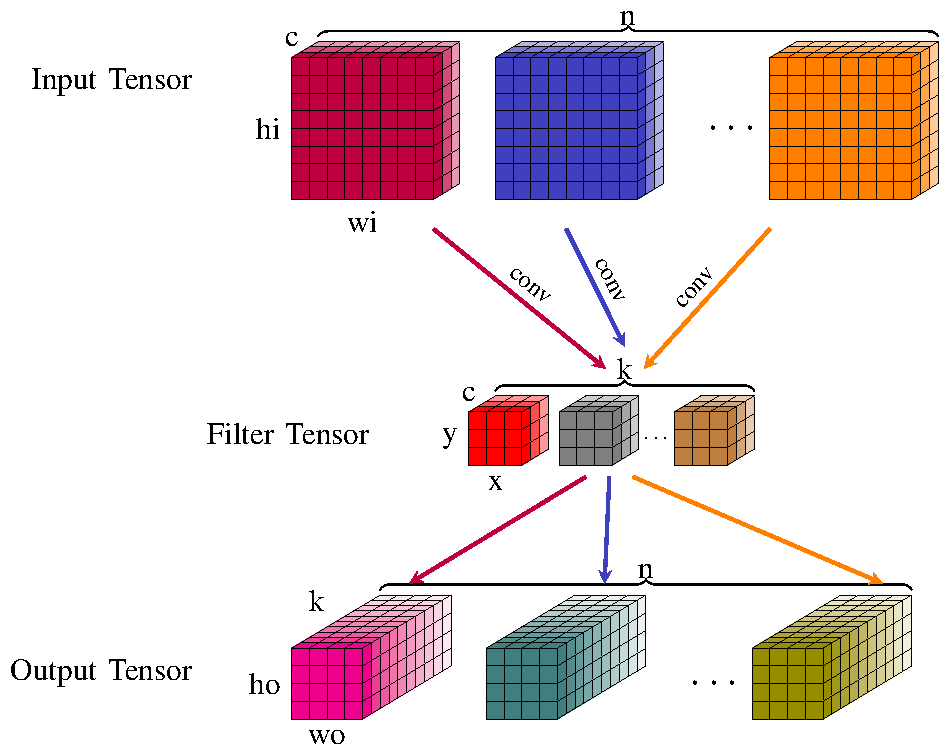
\includegraphics[width=.5\textwidth]{conv2d}
  % \begin{tikzpicture}
  %   \def\unitTensor{0.3}

  %   \def\firstInputCol{purple}
  %   \def\secondInputCol{blue!50!gray}
  %   \def\thirdInputCol{orange}
    
  %   %% input tensor
  %   \def\firstCol{\firstInputCol}
  %   \def\secondCol{\secondInputCol}
  %   \def\thirdCol{\thirdInputCol}
  %   \coordinate (inputTensorTL) at (0,0);
  %   \coordinate (TL) at (inputTensorTL);
  %   \inputTensor{8}{8}{3}{\unitTensor}{hi}{wi}{30}

    
  %   %% filter tensor
  %   \def\firstCol{red}
  %   \def\secondCol{gray}
  %   \def\thirdCol{brown}
  %   \coordinate (filterTensorTL) at (3,-6);
  %   \coordinate (TL) at (filterTensorTL);
  %   \filterTensor{3}{3}{3}{\unitTensor}{30}

  %   \draw [ultra thick, \firstInputCol, ->,>=stealth] ($(firstBR)+(0,-.5)$) -- (labelK.west) node [above, pos=.5, sloped, scale=1.2, black] {conv};
  %   \draw [ultra thick, \secondInputCol, ->,>=stealth] ($(secondmidB)+(0,-.5)$) -- (labelK.north) node [above, pos=.5, sloped, scale=1.2, black] {conv};
  %   \draw [ultra thick, \thirdInputCol, ->,>=stealth] ($(thirdBL)+(0,-.5)$) -- (labelK.east) node [above, pos=.5, sloped, scale=1.2, black] {conv};

  %   %% output tensor
  %   \def\firstCol{magenta}
  %   \def\secondCol{teal!50!gray}
  %   \def\thirdCol{olive}
  %   \def\unitTensor{0.3}
  %   \coordinate (outputTensorTL) at (0, -10);
  %   \coordinate (TL) at (outputTensorTL);
  %   \outputTensor{4}{4}{10}{\unitTensor}{1}{10}

  %   \draw [ultra thick, ->, >=stealth, \firstInputCol] ($(midB.south)+(0,-.2)$) --
  %   ($(backTL1)+(.5,.2)$);
  %   \draw [ultra thick, ->, >=stealth, \secondInputCol] ($(midB.south)+(.4,-.2)$) --
  %   ($(backTL2)+(.5,.2)$);
  %   \draw [ultra thick, ->, >=stealth, \thirdInputCol] ($(midB.south)+(.8,-.2)$) --
  %   ($(backTR3)+(-.5,.2)$);

  %   %% Adding labels
  %   \node [scale=1.5, below left] at ($(inputTensorTL)+(-1.5,0)$) {Input Tensor};
  %   \node [scale=1.5, below left] at ($(filterTensorTL)+(-1.5,0)$) {Filter Tensor};
  %   \node [scale=1.5, below left] at ($(outputTensorTL)+(-1.5,0)$) {Output Tensor};
    
  % \end{tikzpicture}
  \caption{Forward Convolution Diagram}
  \label{fig:conv2d}
\end{figure}

\subsubsection{Filter Tensor}
\Fig \ref{fig:filter_tensor_to_matrix_A} shows the coordinate transformation of
the filter tensor F\{k,c,y,x\} into a matrix A\{gemmM,gemmK\} in a forward convolution.
The c, y, x dimensions in the tensor are merged to form the gemmK dimension in the
matrix.
The k dimension in the tensor is passed through as the gemmM dimension in the matrix.

\hl{TODO: Illustrate how to compute coordinate of the blue element from the matrix
to the tensor in the example.}

% \tikzexternaldisable
\tikzsetnextfilename{filter_tensor_to_matrix_A}
\begin{figure}[!h]
  \centering
  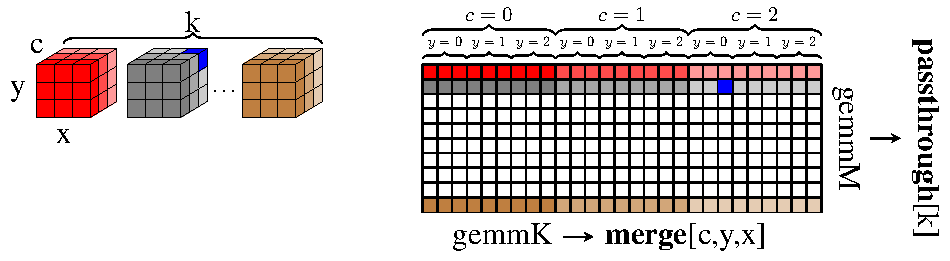
\includegraphics[width=.6\textwidth]{filter_tensor_to_matrix_A}
  % \begin{tikzpicture}
  %   \def\firstCol{red}
  %   \def\secondCol{gray}
  %   \def\thirdCol{brown}
  %   \def\unitMatrix{0.25}
  %   \def\unitTensor{0.3}

  %   \coordinate (TL) at (0,0);
  %   \filterTensor{3}{3}{3}{\unitTensor}{30}
  %   \coordinate (TL) at (secondTL);
  %   \pickElemInTensor{\unitTensor}

  %   \coordinate (matrixTL) at ($(TL)+(5, 0)$);
  %   \coordinate (TL) at (matrixTL);
  %   \filterGemmA{3}{3}{3}{10}{\unitMatrix}{1}
  %   \pickElemInMatrix{1}{20}{\unitMatrix}
  % \end{tikzpicture}
  \caption{Filter tensor F\{k,c,y,x\} to matrix A\{gemmM,gemmK\} in conv2d}
  \label{fig:filter_tensor_to_matrix_A}
\end{figure}


\subsubsection{Input Tensor}
The input tensor goes through a series of transformations to be converted into a matrix.
we first pad the input images along the hi and wi dimensions according to the
padding parameters.
\Fig \ref{fig:input_tensor_to_pad} shows the conversion from the original tensor
X\{n,c,hi,wi\} (left) to a padded tensor X\{n,c,hipad,wipad\} (right) with padding
parameters \{1,1,1,1\}.

\hl{TODO: illustrate how to compute coordinates.}

%\tikzexternaldisable
\tikzsetnextfilename{input_tensor_to_pad}
\begin{figure}[!h]
  \centering
  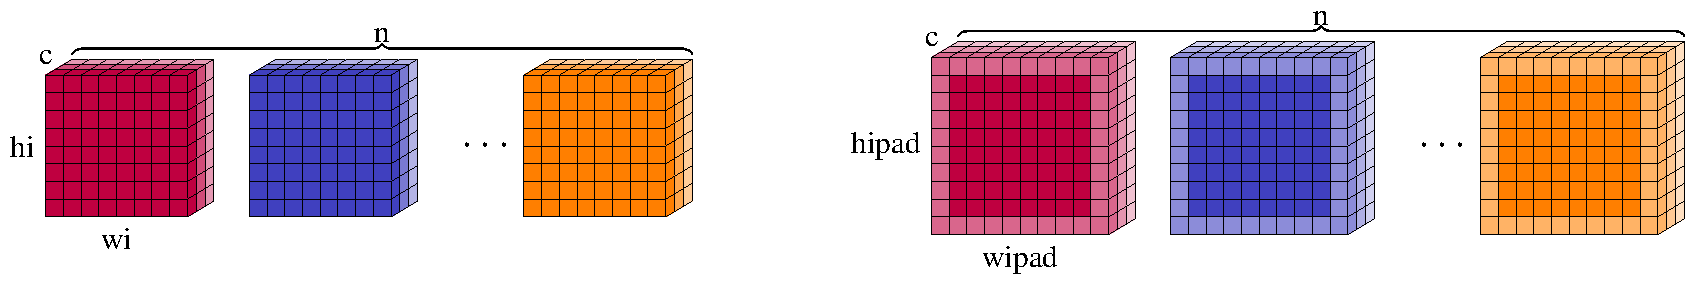
\includegraphics[width=.9\textwidth]{input_tensor_to_pad}
  % \begin{tikzpicture}
  %   \def\firstCol{purple}
  %   \def\secondCol{blue!50!gray}
  %   \def\thirdCol{orange}
  %   \coordinate (TL) at (0,0);
  %   \inputTensor{8}{8}{3}{0.3}{hi}{wi}{30}

  %   %% padded tensor
  %   \def\firstCol{purple!60!white}
  %   \def\secondCol{blue!50!gray!60!white}
  %   \def\thirdCol{orange!60!white}
  %   \coordinate (PadTL) at ($(TL)+(15,.3)$);
  %   \coordinate (TL) at (PadTL);
  %   \inputTensor{10}{10}{3}{0.3}{hipad}{wipad}{30}
  %   \inputTensorPad{8}{8}{0.3}
  % \end{tikzpicture}
  \caption{Input tensor X\{n,c,hi,wi\} (left) and
    after padding $\text{Pad}\{1,1,1,1\}[hipad,wipad] \leftarrow [hi,wi]$ (right)}
  \label{fig:input_tensor_to_pad}
\end{figure}


% \tikzexternaldisable
% \tikzsetnextfilename{input_pad_tensor}
% \begin{figure}[!h]
%   \centering
%   %\includegraphics[width=.4\textwidth]{input_pad_tensor}
%   \begin{tikzpicture}
%     \def\firstCol{purple!60!white}
%     \def\secondCol{blue!50!gray!60!white}
%     \def\thirdCol{orange!60!white}
%     \coordinate (PadTL) at (0,0);
%     \coordinate (TL) at (PadTL);
%     \inputTensor{10}{10}{3}{0.3}{hipad}{wipad}{30}
%     \inputTensorPad{8}{8}{0.3}
%   \end{tikzpicture}
%   \caption{Input tensor after padding $\text{Pad}\{1,1,1,1\}[hipad,wipad] \leftarrow [hi,wi]$}
%   \label{fig:input_pad_tensor}
% \end{figure}

Then we break down the input images (\{c, hipad, wipad\}) into sub-images (\{c,y,x\})
consisting of pixels that are corresponding to the filter tensor, as shown in
\Fig \ref{fig:input_embed_tensor}.
This process is performed according to the stride and dilation parameters.

\hl{TODO: add more details about the coordinate computation of the embed transform.}

\tikzsetnextfilename{input_embed_tensor}
\begin{figure}[!h]
  \centering
  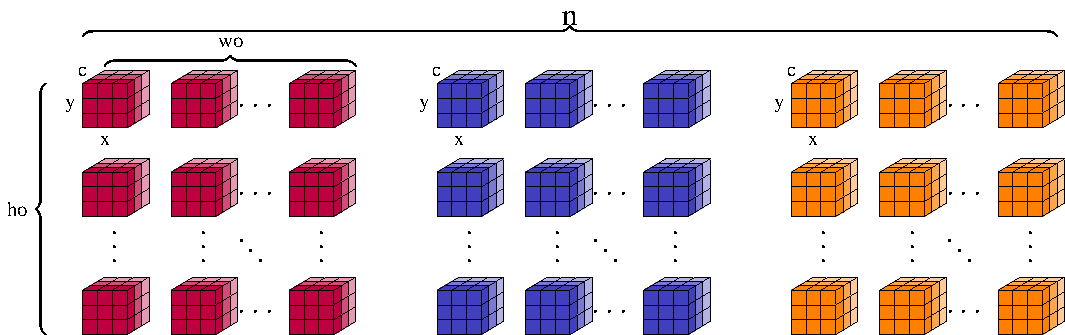
\includegraphics[width=.9\textwidth]{input_embed_tensor}
  % \begin{tikzpicture}
  %   \def\firstCol{purple}
  %   \def\secondCol{blue!50!gray}
  %   \def\thirdCol{orange}
  %   \coordinate (EmbedTL) at (0,0);
  %   \coordinate (TL) at (EmbedTL);
  %   \inputTensorAfterEmbed{3}{3}{3}{0.25}{30}
  % \end{tikzpicture}
  \caption{Input tensor after embedding Embed\{strideH, dilationH\}[ho,y] $\leftarrow$ [hipad] and Embed\{strideW, dilationW\}[wo,x] $\leftarrow$ [wipad]}
  \label{fig:input_embed_tensor}
\end{figure}

At last, the sub-images can be flattened into a matrix as shown in
\Fig \ref{fig:input_matrix_B}.
The c, y, x dimensions in the tensor are merged to form the gemmK dimension
in the matrix.
The n, ho, wo dimensions in the tensor are merged to form the gemmN
dimension in the matrix.
%\tikzexternaldisable
\tikzsetnextfilename{input_matrix_B}
\begin{figure}[!h]
  \centering
  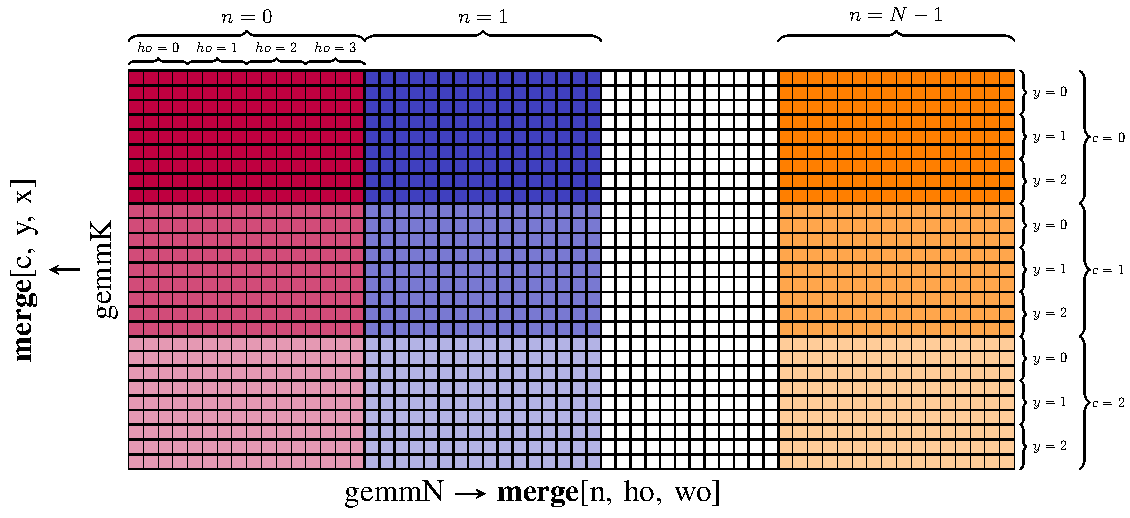
\includegraphics[width=.6\textwidth]{input_matrix_B}
  % \begin{tikzpicture}
  %   \def\firstCol{purple}
  %   \def\secondCol{blue!50!gray}
  %   \def\thirdCol{orange}
  %   \coordinate (inputGemmTL) at (0,0);
  %   \coordinate (TL) at (inputGemmTL);
  %   \inputGemmB{3}{3}{3}{60}{4}{4}{0.25}{1}
  % \end{tikzpicture}
  \caption{Input matrix B\{gemmK,gemmN\}}
  \label{fig:input_matrix_B}
\end{figure}


\subsubsection{Output Tensor}

The output tensor is flattened into a matrix as shown in
\Fig \ref{fig:output_tensor_to_matrix_C}.
The n, ho, wo dimensions in the tensor are merged to form the gemmM dimension
in the matrix.
The k dimension in the tensor is passed through as the gemmN dimension in
the matrix.

%\tikzexternaldisable
\tikzsetnextfilename{output_tensor_to_matrix_C}
\begin{figure}[!h]
  \centering
  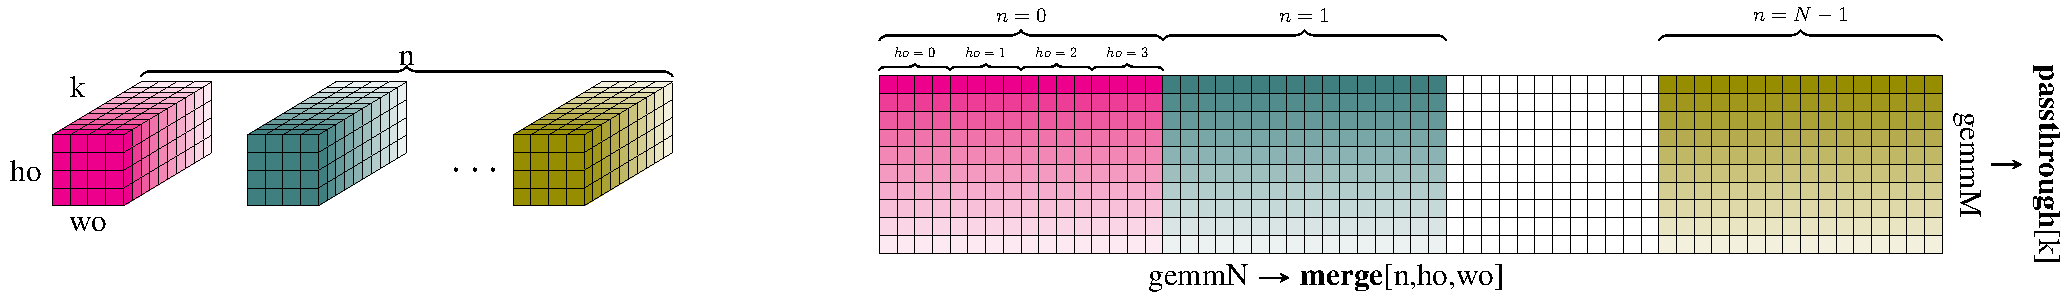
\includegraphics[width=\textwidth]{output_tensor_to_matrix_C}
  % \begin{tikzpicture}
  %   \def\firstCol{magenta}
  %   \def\secondCol{teal!50!gray}
  %   \def\thirdCol{olive}
  %   \def\unitTensor{0.3}
  %   \coordinate (outputTensorTL) at (0,0);
  %   \coordinate (TL) at (outputTensorTL);
  %   \outputTensor{4}{4}{10}{\unitTensor}{1}{10}

  %   %% output gemm C
  %   \def\unitMatrix{0.3}
  %   \coordinate (outputMatrixTL) at ($(outputTensorTL)+(14,1)$);
  %   \coordinate (TL) at (outputMatrixTL);
  %   \outputGemmC{10}{60}{4}{4}{\unitMatrix}{10}{1}
  % \end{tikzpicture}
  \caption{Output tensor O\{n,k,ho,wo\} to matrix C\{gemmM,gemmN\}}
  \label{fig:output_tensor_to_matrix_C}
\end{figure}


%\tikzexternaldisable
% \tikzsetnextfilename{output_matrix_C}
% \begin{figure}[!h]
%   \centering
%   \begin{tikzpicture}[scale=.9]
%     \def\firstCol{magenta}
%     \def\secondCol{teal!50!gray}
%     \def\thirdCol{olive}
%     \def\unitMatrix{0.3}
%     \coordinate (outputMatrixTL) at (0,0);
%     \coordinate (TL) at (outputMatrixTL);
%     \outputGemmC{10}{60}{4}{4}{\unitMatrix}{10}{1}
    
%   \end{tikzpicture}
%   \caption{Output matrix C\{gemmM,gemmN\}}
%   \label{fig:output_matrix_C}
% \end{figure}


\subsubsection{The Transformed Gemm}

The forward convolution is converted into a gemm as shown in
\Fig \ref{fig:conv2d_GEMM}.

%\tikzexternaldisable
\tikzsetnextfilename{conv2d_gemm}
\begin{figure}[!h]
  \centering
  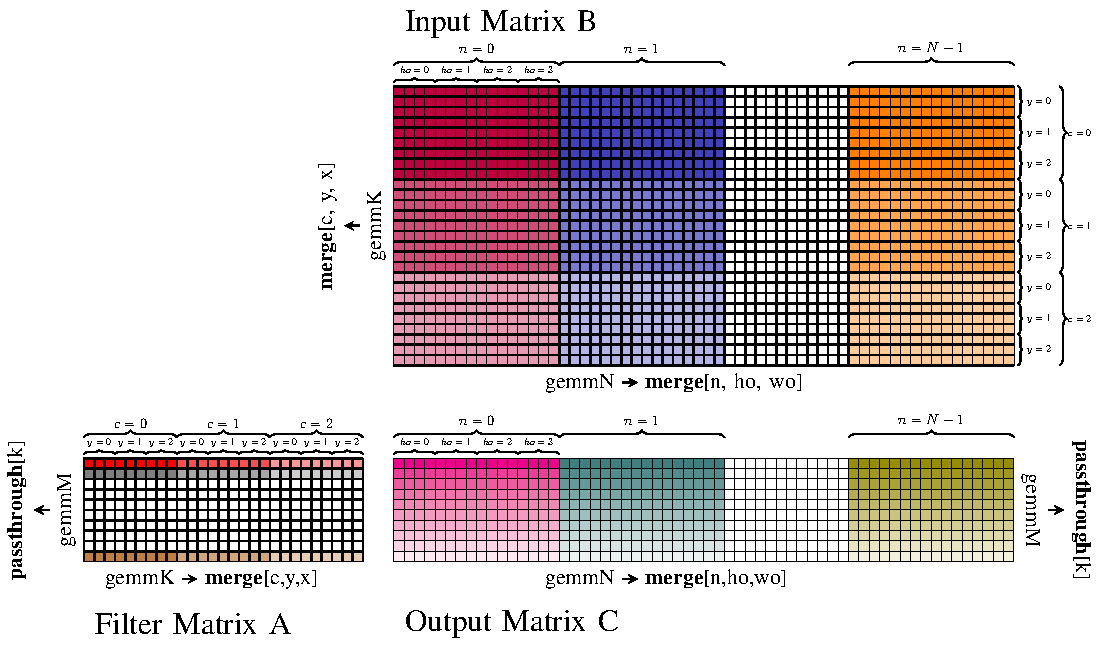
\includegraphics[width=.9\textwidth]{conv2d_gemm}
  % \begin{tikzpicture}[scale=.7]
  %   %% filter matrix
  %   \def\firstCol{red}
  %   \def\secondCol{gray}
  %   \def\thirdCol{brown}
  %   \def\unitMatrix{0.25}
  %   \coordinate (filterGemmTL) at (0,0);
  %   \coordinate (TL) at (filterGemmTL);
  %   \filterGemmA{3}{3}{3}{10}{\unitMatrix}{.7}
  %   %\pickElemInMatrix{1}{20}{\unitMatrix}

  %   %% input matrix
  %   \def\firstCol{purple}
  %   \def\secondCol{blue!50!gray}
  %   \def\thirdCol{orange}
  %   \coordinate (inputGemmTL) at (7.5,9);
  %   \coordinate (TL) at (inputGemmTL);
  %   \inputGemmB{3}{3}{3}{60}{4}{4}{\unitMatrix}{.7}

  %   %% output matrix
  %   \def\firstCol{magenta}
  %   \def\secondCol{teal!50!gray}
  %   \def\thirdCol{olive}
  %   \coordinate (outputGemmTL) at (7.5,0);
  %   \coordinate (TL) at (outputGemmTL);
  %   \outputGemmC{10}{60}{4}{4}{\unitMatrix}{10}{.7}

  %   %% labels
  %   \node [scale=1.5,right] at ($(filterGemmTL)+(0,-4)$) {Filter Matrix A};
  %   \node [scale=1.5,right] at ($(inputGemmTL)+(0,1.5)$) {Input Matrix B};
  %   \node [scale=1.5,right] at ($(outputGemmTL)+(0,-4)$) {Output Matrix C};
  % \end{tikzpicture}
  \caption{GEMM for conv2d}
  \label{fig:conv2d_GEMM}
\end{figure}


\subsection{Backward Weight Convolution, i.e. $\partial \bold{L}/\partial \bold{F}$}
The backward weight convolution refers to the step to compute $\partial \bold{L}/\partial \bold{F}$
during back-propagation.
As shown in \Fig \ref{fig:conv2d_bwd_weight_gemm}, each image in the input batch is convoluted
with its corresponding output image to produce one filter.
And all the filters are summed to produce the final filter gradient $\partial \bold{L}/\partial \bold{F}$.

The transformations of input, filter, and output tensors into matrices are very similar to
the forward convolution case.
The only difference is that some matrices need to be transposed.
%\Fig \ref{fig:output_matrix_A_conv2d_bwd_weight}, \ref{fig:input_matrix_B_con2d_bwd_weight},
%and \ref{fig:filter_matrix_C}.

%\tikzexternaldisable
% \tikzsetnextfilename{conv2d_bwd_weight}
% \begin{figure}[!h]
%   \centering
%   \begin{tikzpicture}
%     \def\unitTensor{0.3}

%     \def\firstInputCol{purple}
%     \def\secondInputCol{blue!50!gray}
%     \def\thirdInputCol{orange}
    
%     %% input tensor
%     \def\firstCol{\firstInputCol}
%     \def\secondCol{\secondInputCol}
%     \def\thirdCol{\thirdInputCol}
%     \coordinate (inputTensorTL) at (0,0);
%     \coordinate (TL) at (inputTensorTL);
%     \inputTensor{8}{8}{3}{\unitTensor}{hi}{wi}{30}

%     %% output tensor
%     \def\firstCol{magenta}
%     \def\secondCol{teal!50!gray}
%     \def\thirdCol{olive}
%     \def\unitTensor{0.3}
%     \coordinate (outputTensorTL) at (0, -6);
%     \coordinate (TL) at (outputTensorTL);
%     \outputTensor{4}{4}{10}{\unitTensor}{1}{10}


%     \draw [ultra thick, \firstInputCol, ->,>=stealth] ($(firstBR)+(-4*\unitTensor,-.8)$) -- ++(0, -1.5) node [above, pos=.5, sloped, scale=1.2, black] {conv};
%     \draw [ultra thick, \secondInputCol, ->,>=stealth] ($(secondmidB)+(0,-.5)$) -- ++(0, -1.8) node [above, pos=.5, sloped, scale=1.2, black] {conv};
%     \draw [ultra thick, \thirdInputCol, ->,>=stealth] ($(thirdBL)+(4*\unitTensor,-.5)$) -- ++(0, -1.8) node [above, pos=.5, sloped, scale=1.2, black] {conv};

%     %% filter tensor
%     \def\firstCol{red}
%     \def\secondCol{gray}
%     \def\thirdCol{brown}
%     \coordinate (filterTensorTL) at (-4,-10);
%     \coordinate (TL) at (filterTensorTL);
%     \filterTensor{3}{3}{3}{\unitTensor}{30}
%     \draw [ultra thick, ->, >=stealth, \firstInputCol] ($(midB1)+(0, -.5)$) -- (labelK);

%     \coordinate (TL) at ($(TL)+(6,0)$);
%     \filterTensor{3}{3}{3}{\unitTensor}{30}
%     \draw [ultra thick, ->, >=stealth, \secondInputCol] ($(midB2)+(0, -.2)$) -- (labelK);
    
%     \coordinate (TL) at ($(TL)+(7,0)$);
%     \filterTensor{3}{3}{3}{\unitTensor}{30}
%     \draw [ultra thick, ->, >=stealth, \thirdInputCol] ($(midB3)+(0, -.2)$) -- (labelK);
%     \node [left, scale=2] at ($(TL)+(-.5, -1.5*\unitTensor)$) {$\cdots$};

%     \coordinate (filterTensorTL) at (3,-14);
%     \coordinate (TL) at (filterTensorTL);
%     \filterTensor{3}{3}{3}{\unitTensor}{30}
%     \draw [ultra thick, <-, >=stealth] (labelK) -- ++(0, 1.5)
%     node [pos=.5, right, scale=1.2] {sum};

%     %% Adding labels
%     \node [scale=1.5, below left] at ($(inputTensorTL)+(-1.5,0)$) {Input Tensor};
%     \node [scale=1.5, below left, align=center] at ($(filterTensorTL)+(-1.5,0)$)
%     {Filter Loss\\
%       Gradient $\bold{\frac{\partial L}{\partial F}}$};
%     \node [scale=1.5, below left, align=center] at ($(outputTensorTL)+(-1.5,0)$)
%     {Output Loss\\
%       Gradient $\bold{\frac{\partial L}{\partial O}}$};
    
%   \end{tikzpicture}
%   \caption{Backward weight convolution diagram}
%   \label{fig:conv2d_bwd_weight}
% \end{figure}

% \tikzexternaldisable
% \tikzsetnextfilename{output_matrix_A_conv2d_bwd_weight}
% \begin{figure}[!h]
%   \centering
%   \begin{tikzpicture}[scale=.9]
%     \def\firstCol{magenta}
%     \def\secondCol{teal!50!gray}
%     \def\thirdCol{olive}
%     \def\unitMatrix{0.3}
%     \coordinate (outputMatrixTL) at (0,0);
%     \coordinate (TL) at (outputMatrixTL);
%     \outputGemmA{10}{60}{4}{4}{\unitMatrix}{10}{.9}
%   \end{tikzpicture}
%   \caption{Output matrix A\{gemmM,gemmK\} for conv2d\_bwd\_weight}
%   \label{fig:output_matrix_A_conv2d_bwd_weight}
% \end{figure}

% %\tikzexternaldisable
% \tikzsetnextfilename{input_matrix_B_conv2d_bwd_weight}
% \begin{figure}[!h]
%   \centering
%   \begin{tikzpicture}
%     \def\firstCol{purple}
%     \def\secondCol{blue!50!gray}
%     \def\thirdCol{orange}
%     \coordinate (inputGemmTL) at (0,0);
%     \coordinate (TL) at (inputGemmTL);
%     \inputGemmBBwdWeight{3}{3}{3}{60}{4}{4}{0.25}{1}
%   \end{tikzpicture}
%   \caption{Input matrix B\{gemmK,gemmN\} for conv2d\_bwd\_weight}
%   \label{fig:input_matrix_B_con2d_bwd_weight}
% \end{figure}

% %\tikzexternaldisable
% \tikzsetnextfilename{filter_matrix_C}
% \begin{figure}[!h]
%   \centering
%   \begin{tikzpicture}
%     \def\firstCol{red}
%     \def\secondCol{gray}
%     \def\thirdCol{brown}
%     \def\unitMatrix{0.25}
%     \coordinate (TL) at (0,0);
%     \filterGemmC{3}{3}{3}{10}{\unitMatrix}{1}
%     %\pickElemInMatrix{1}{20}{\unitMatrix}
%   \end{tikzpicture}
%   \caption{Filter matrix C\{gemmM,gemmN\}}
%   \label{fig:filter_matrix_C}
% \end{figure}


%\subsubsection{ConvToGemm}

\Fig \ref{fig:conv2d_bwd_weight_gemm} shows the transformed gemm from backward weight
convolution.

In general, the batch size n is large enough so that we can benefit from partitioning
matrix A and B into sub-batches, which can be computed in parallel.
However, the hardware needs to support atomic add so that the values in matrix C
can be updated correctly.

%\tikzexternaldisable
\tikzsetnextfilename{conv2d_bwd_weight_gemm}
\begin{figure}[!h]
  \centering
  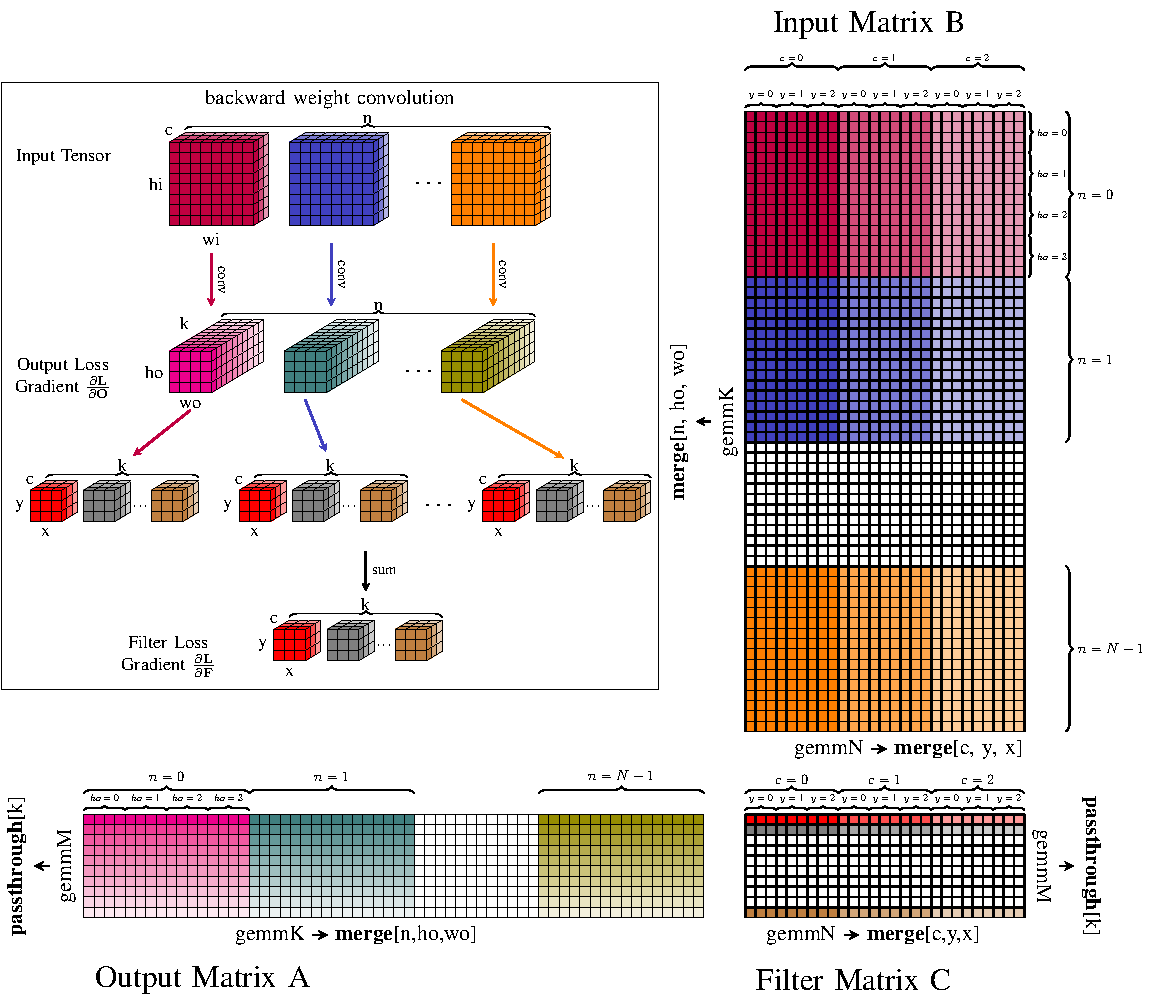
\includegraphics[width=\textwidth]{conv2d_bwd_weight_gemm}
  % \begin{tikzpicture}[scale=.7]
  %   %% output matrix
  %   \def\firstCol{magenta}
  %   \def\secondCol{teal!50!gray}
  %   \def\thirdCol{olive}
  %   \def\unitMatrix{0.25}
  %   \coordinate (outputGemmTL) at (0,0);
  %   \coordinate (TL) at (outputGemmTL);
  %   \outputGemmA{10}{60}{4}{4}{\unitMatrix}{10}{.7}

  %   %% Input matrix
  %   \def\firstCol{purple}
  %   \def\secondCol{blue!50!gray}
  %   \def\thirdCol{orange}
  %   \coordinate (inputGemmTL) at (16,17);
  %   \coordinate (TL) at (inputGemmTL);
  %   \inputGemmBBwdWeight{3}{3}{3}{60}{4}{4}{\unitMatrix}{.7}

  %   %% Filter matrix
  %   \def\firstCol{red}
  %   \def\secondCol{gray}
  %   \def\thirdCol{brown}
  %   \coordinate (filterGemmTL) at (16,0);
  %   \coordinate (TL) at (filterGemmTL);
  %   \filterGemmC{3}{3}{3}{10}{\unitMatrix}{.7}

  %   %% labels
  %   \node [scale=1.5,right] at ($(outputGemmTL)+(0,-4)$) {Output Matrix A};
  %   \node [scale=1.5,above] at ($(inputGemmTL)+(3,1.5)$) {Input Matrix B};
  %   \node [scale=1.5,right] at ($(filterGemmTL)+(0,-4)$) {Filter Matrix C};

  %   %% Insert the conv2d_bwd_weight diagram as an image
  %   \node [draw=black, above right, align=center] at (-2,3) {
  %     backward weight convolution\\
  %     \includegraphics[width=.6\textwidth]{conv2d_bwd_weight}
  %   };

  % \end{tikzpicture}
  \caption{Conversion from conv2d\_bwd\_weight to gemm.}
  \label{fig:conv2d_bwd_weight_gemm}
\end{figure}

%\tikzexternaldisable
%\tikzsetnextfilename{input_tensor}
% \begin{figure}[!h]
%   \centering
%   \begin{tikzpicture}
%     \def\firstCol{purple}
%     \def\secondCol{blue!50!gray}
%     \def\thirdCol{orange}
%     \coordinate (TL) at (0,0);
%     \coordinate (origTL) at (TL);
%     \inputTensor{8}{8}{3}{0.3}{$``hi"$}{$``wi"$}

%     \draw [->,>=stealth, ultra thick] ($(TL)+(5,-2.5)$) -- ++(0, -1)
%     node [right, scale=1.5, pos=0.5] {Pad\{1,1,1,1\}[$``hi"$, $``wi"$]};
    
    
%     \def\firstCol{purple!60!white}
%     \def\secondCol{blue!50!gray!60!white}
%     \def\thirdCol{orange!60!white}
%     \coordinate (PadTL) at ($(origTL)+(-1,-4.5)$);
%     \coordinate (TL) at (PadTL);
%     \inputTensor{10}{10}{3}{0.3}{$``hipad"$}{$``wipad"$}
%     \inputTensorPad{8}{8}{0.3}


%     \draw [->,>=stealth, ultra thick] ($(origTL)+(5,-8)$) -- ++(0, -1)
%     node [right, scale=1.5, pos=0.5] {Embed\{1,1\}[$``hipad"$]\{1,1\}[$``wipad"$]};
    
    
%     \def\firstCol{purple}
%     \def\secondCol{blue!50!gray}
%     \def\thirdCol{orange}
%     \coordinate (EmbedTL) at ($(PadTL)+(-2, -5)$);
%     \coordinate (TL) at (EmbedTL);
%     \inputTensorAfterEmbed{3}{3}{3}{0.25}

%     \coordinate (inputGemmTL) at ($(EmbedTL)+(1, -6)$);
%     \coordinate (TL) at (inputGemmTL);
%     \inputGemmB{3}{3}{3}{60}{4}{4}{0.25}

%     %% The inputGemm
%   \end{tikzpicture}
%   \caption{Coordinate transformation of input tensor $\{``n",``c",``hi",``wi"\}$}
%   \label{fig:input_tensor}
% \end{figure}

\subsection{Backward Data, i.e. $\partial \bold{L}/\partial \bold{X}$}
We use the v4r1 algorithm to implement the backward data convolution.
\hl{TODO: Understand and explain the algorithm.}

% Using the chain rule, we can have
% \begin{equation}\label{eq:chain_rule_for_X}
%   \frac{\partial \bold{L}}{\partial \bold{X}} = \frac{\partial \bold{L}}{\partial \bold{O}} \times \frac{\partial \bold{O}}{\partial \bold{X}}
% \end{equation}
% $\partial \bold{L}/\partial \bold{O}$ is the loss gradient from the previous layer.


% %\tikzexternaldisable
% \tikzsetnextfilename{2d_fwd_conv_simple}
% \begin{figure}[!h]
%   \centering
%   \begin{tikzpicture}
%     \def\cellUnit{0.8}
%     \coordinate (TL) at (0,0);
%     \drawMatrix{4}{4}{\cellUnit}{X}{0}{1}
%     \coordinate (labelInput) at ($(TL)+(2*\cellUnit, -4.5*\cellUnit)$);
%     \coordinate (labelFilter) at ($(labelInput)+(5*\cellUnit, 0)$);
%     \coordinate (labelOutput) at ($(labelFilter)+(4.5*\cellUnit, 0)$);

%     \draw [ultra thick, ->, >=stealth, white] ($(TL)+(4*\cellUnit+.1, -2*\cellUnit)$)
%     -- ++(2*\cellUnit-.2, 0) node [pos=.5, black] {conv};

%     \coordinate (TL) at ($(TL)+(6*\cellUnit,-\cellUnit)$);
%     \drawMatrix{2}{2}{\cellUnit}{F}{0}{1}

%     \draw [ultra thick, ->, >=stealth, white] ($(TL)+(2*\cellUnit+.1, -1*\cellUnit)$)
%     -- ++(2*\cellUnit-.2, 0) node [pos=.5, scale=1.5, black] {=};

%     \coordinate (TL) at ($(TL)+(4*\cellUnit,0.5*\cellUnit)$);
%     \drawMatrix{3}{3}{\cellUnit}{O}{0}{1}

%     %% labels
%     \node [scale=1.5] at (labelInput) {Input};
%     \node [scale=1.5] at (labelFilter) {Filter};
%     \node [scale=1.5] at (labelOutput) {Output};
%   \end{tikzpicture}
%   \caption{Forward convolution without considering channels. stride = dilation = 1}
%   \label{fig:2d_fwd_conv_simple}
% \end{figure}

% \Fig \ref{fig:2d_fwd_conv_simple} shows a very simple illustration of a forward convolution.

% \begin{align}\label{eq:conv2d_fwd_output}
%   \bold{O}_{11} & = \bold{X}_{11} \times \bold{F}_{11} + \bold{X}_{12} \times \bold{F}_{12}
%                   + \bold{X}_{21} \times \bold{F}_{21} + \bold{X}_{22} \times \bold{F}_{22} \\
%   \bold{O}_{12} & = \bold{X}_{12} \times \bold{F}_{11} + \bold{X}_{13} \times \bold{F}_{12}
%                   + \bold{X}_{22} \times \bold{F}_{21} + \bold{X}_{23} \times \bold{F}_{22} \\
%   \bold{O}_{13} & = \bold{X}_{13} \times \bold{F}_{11} + \bold{X}_{14} \times \bold{F}_{12}
%                   + \bold{X}_{23} \times \bold{F}_{21} + \bold{X}_{24} \times \bold{F}_{22} \\
%   \bold{O}_{21} & = \bold{X}_{21} \times \bold{F}_{11} + \bold{X}_{22} \times \bold{F}_{12}
%                   + \bold{X}_{31} \times \bold{F}_{21} + \bold{X}_{32} \times \bold{F}_{22} \\
%   \bold{O}_{22} & = \bold{X}_{22} \times \bold{F}_{11} + \bold{X}_{23} \times \bold{F}_{12}
%                   + \bold{X}_{32} \times \bold{F}_{21} + \bold{X}_{33} \times \bold{F}_{22}\\
%   \bold{O}_{23} & = \bold{X}_{23} \times \bold{F}_{11} + \bold{X}_{24} \times \bold{F}_{12}
%                   + \bold{X}_{33} \times \bold{F}_{21} + \bold{X}_{34} \times \bold{F}_{22}\\
%   \bold{O}_{31} & = \bold{X}_{31} \times \bold{F}_{11} + \bold{X}_{32} \times \bold{F}_{12}
%                   + \bold{X}_{41} \times \bold{F}_{21} + \bold{X}_{42} \times \bold{F}_{22}\\
%   \bold{O}_{32} & = \bold{X}_{32} \times \bold{F}_{11} + \bold{X}_{33} \times \bold{F}_{12}
%                   + \bold{X}_{42} \times \bold{F}_{21} + \bold{X}_{43} \times \bold{F}_{22}\\
%   \bold{O}_{33} & = \bold{X}_{33} \times \bold{F}_{11} + \bold{X}_{34} \times \bold{F}_{12}
%                    + \bold{X}_{43} \times \bold{F}_{21} + \bold{X}_{44} \times \bold{F}_{22}
% \end{align}

% Local gradients for X is

% \begin{align}\label{eq:local_gradients_X}
%   \frac{\partial \bold{O}_{11}}{\partial \bold{X}_{11}} = \bold{F}_{11}\;\;\;\;
%   \frac{\partial \bold{O}_{11}}{\partial \bold{X}_{12}} = \bold{F}_{12}\;\;\;\;
%   \frac{\partial \bold{O}_{11}}{\partial \bold{X}_{21}} = \bold{F}_{21}\;\;\;\;
%   \frac{\partial \bold{O}_{11}}{\partial \bold{X}_{22}} = \bold{F}_{22}\;\;\;\;\\
%   \frac{\partial \bold{O}_{12}}{\partial \bold{X}_{12}} = \bold{F}_{11}\;\;\;\;
%   \frac{\partial \bold{O}_{12}}{\partial \bold{X}_{13}} = \bold{F}_{12}\;\;\;\;
%   \frac{\partial \bold{O}_{12}}{\partial \bold{X}_{22}} = \bold{F}_{21}\;\;\;\;
%   \frac{\partial \bold{O}_{12}}{\partial \bold{X}_{23}} = \bold{F}_{22}\;\;\;\;\\
%   \frac{\partial \bold{O}_{13}}{\partial \bold{X}_{13}} = \bold{F}_{11}\;\;\;\;
%   \frac{\partial \bold{O}_{13}}{\partial \bold{X}_{14}} = \bold{F}_{12}\;\;\;\;
%   \frac{\partial \bold{O}_{13}}{\partial \bold{X}_{23}} = \bold{F}_{21}\;\;\;\;
%   \frac{\partial \bold{O}_{13}}{\partial \bold{X}_{24}} = \bold{F}_{22}\;\;\;\;\\
%   \frac{\partial \bold{O}_{21}}{\partial \bold{X}_{21}} = \bold{F}_{11}\;\;\;\;
%   \frac{\partial \bold{O}_{21}}{\partial \bold{X}_{22}} = \bold{F}_{12}\;\;\;\;
%   \frac{\partial \bold{O}_{21}}{\partial \bold{X}_{31}} = \bold{F}_{21}\;\;\;\;
%   \frac{\partial \bold{O}_{21}}{\partial \bold{X}_{32}} = \bold{F}_{22}\;\;\;\;\\
%   \frac{\partial \bold{O}_{22}}{\partial \bold{X}_{22}} = \bold{F}_{11}\;\;\;\;
%   \frac{\partial \bold{O}_{22}}{\partial \bold{X}_{23}} = \bold{F}_{12}\;\;\;\;
%   \frac{\partial \bold{O}_{22}}{\partial \bold{X}_{32}} = \bold{F}_{21}\;\;\;\;
%   \frac{\partial \bold{O}_{22}}{\partial \bold{X}_{33}} = \bold{F}_{22}\;\;\;\;\\
%   \frac{\partial \bold{O}_{23}}{\partial \bold{X}_{23}} = \bold{F}_{11}\;\;\;\;
%   \frac{\partial \bold{O}_{23}}{\partial \bold{X}_{24}} = \bold{F}_{12}\;\;\;\;
%   \frac{\partial \bold{O}_{23}}{\partial \bold{X}_{33}} = \bold{F}_{21}\;\;\;\;
%   \frac{\partial \bold{O}_{23}}{\partial \bold{X}_{34}} = \bold{F}_{22}\;\;\;\;\\
%   \frac{\partial \bold{O}_{31}}{\partial \bold{X}_{31}} = \bold{F}_{11}\;\;\;\;
%   \frac{\partial \bold{O}_{31}}{\partial \bold{X}_{32}} = \bold{F}_{12}\;\;\;\;
%   \frac{\partial \bold{O}_{31}}{\partial \bold{X}_{41}} = \bold{F}_{21}\;\;\;\;
%   \frac{\partial \bold{O}_{31}}{\partial \bold{X}_{42}} = \bold{F}_{22}\;\;\;\;\\
%   \frac{\partial \bold{O}_{32}}{\partial \bold{X}_{32}} = \bold{F}_{11}\;\;\;\;
%   \frac{\partial \bold{O}_{32}}{\partial \bold{X}_{33}} = \bold{F}_{12}\;\;\;\;
%   \frac{\partial \bold{O}_{32}}{\partial \bold{X}_{42}} = \bold{F}_{21}\;\;\;\;
%   \frac{\partial \bold{O}_{32}}{\partial \bold{X}_{43}} = \bold{F}_{22}\;\;\;\;\\
%   \frac{\partial \bold{O}_{33}}{\partial \bold{X}_{33}} = \bold{F}_{11}\;\;\;\;
%   \frac{\partial \bold{O}_{33}}{\partial \bold{X}_{34}} = \bold{F}_{12}\;\;\;\;
%   \frac{\partial \bold{O}_{33}}{\partial \bold{X}_{43}} = \bold{F}_{21}\;\;\;\;
%   \frac{\partial \bold{O}_{33}}{\partial \bold{X}_{44}} = \bold{F}_{22}\;\;\;\;\\
% \end{align}

% Let's set
% \begin{equation}
%   \frac{\partial \bold{L}}{\partial \bold{O}_{ij}} = \bold{L}_{ij}
% \end{equation}
% And we also have
% \begin{align}\label{eq:gradient_X}
%   \frac{\partial \bold{L}}{\partial \bold{X}_{ij}}=\sum_k\bold{L}_{k}\times\frac{\partial \bold{O}_k}{\partial \bold{X}_{ij}}
% \end{align}

% Then we can get the X gradient

% \begin{align}
%   \frac{\partial \bold{L}}{\partial \bold{X}_{11}} &= \bold{L}_{11}\times \bold{F}_{11} \\
%   \frac{\partial \bold{L}}{\partial \bold{X}_{12}} &= \bold{L}_{11}\times \bold{F}_{12} +  \bold{L}_{12}\times \bold{F}_{11}\\
%   \frac{\partial \bold{L}}{\partial \bold{X}_{13}} &= \bold{L}_{12}\times \bold{F}_{12} +  \bold{L}_{13}\times \bold{F}_{11}\\
%   \frac{\partial \bold{L}}{\partial \bold{X}_{14}} &= \bold{L}_{13}\times \bold{F}_{12}
% \end{align}

% \begin{align}
%   \frac{\partial \bold{L}}{\partial \bold{X}_{21}} &= \bold{L}_{11}\times \bold{F}_{21} + \bold{L}_{21}\times \bold{F}_{11} \\
%   \frac{\partial \bold{L}}{\partial \bold{X}_{22}} &= \bold{L}_{11}\times \bold{F}_{22} + \bold{L}_{12}\times \bold{F}_{21} + \bold{L}_{21}\times \bold{F_{12}} + \bold{L}_{22}\times \bold{F_{11}}\\
%   \frac{\partial \bold{L}}{\partial \bold{X}_{23}} &= \bold{L}_{12}\times \bold{F}_{22} + \bold{L}_{13}\times \bold{F}_{21} + \bold{L}_{22}\times \bold{F_{12}} + \bold{L}_{23}\times \bold{F_{11}}\\
%   \frac{\partial \bold{L}}{\partial \bold{X}_{24}} &= \bold{L}_{13}\times \bold{F}_{22} + \bold{L}_{23}\times \bold{F}_{12}\\
% \end{align}

% \begin{align}
%   \frac{\partial \bold{L}}{\partial \bold{X}_{31}} &= \bold{L}_{21}\times \bold{F}_{21} + \bold{L}_{31}\times \bold{F}_{11} \\
%   \frac{\partial \bold{L}}{\partial \bold{X}_{32}} &= \bold{L}_{21}\times \bold{F}_{22} + \bold{L}_{22}\times \bold{F}_{21} + \bold{L}_{31}\times \bold{F_{12}} + \bold{L}_{32}\times \bold{F_{11}}\\
%   \frac{\partial \bold{L}}{\partial \bold{X}_{33}} &= \bold{L}_{22}\times \bold{F}_{22} + \bold{L}_{23}\times \bold{F}_{21} + \bold{L}_{32}\times \bold{F_{12}} + \bold{L}_{33}\times \bold{F_{11}}\\
%   \frac{\partial \bold{L}}{\partial \bold{X}_{34}} &= \bold{L}_{23}\times \bold{F}_{22} + \bold{L}_{33}\times \bold{F}_{12}\\
% \end{align}

% \begin{align}
%   \frac{\partial \bold{L}}{\partial \bold{X}_{41}} &= \bold{L}_{31}\times \bold{F}_{21} \\
%   \frac{\partial \bold{L}}{\partial \bold{X}_{42}} &= \bold{L}_{31}\times \bold{F}_{22} +  \bold{L}_{32}\times \bold{F}_{21}\\
%   \frac{\partial \bold{L}}{\partial \bold{X}_{43}} &= \bold{L}_{32}\times \bold{F}_{32} +  \bold{L}_{33}\times \bold{F}_{21}\\
%   \frac{\partial \bold{L}}{\partial \bold{X}_{44}} &= \bold{L}_{33}\times \bold{F}_{22}
% \end{align}



% \tikzexternaldisable
% %\tikzsetnextfilename{2d_bwd_data}
% \begin{figure}[!h]
%   \centering
%   \begin{tikzpicture}
%     \def\cellUnit{0.8}
%     \coordinate (TL) at (0,0);
%     \drawMatrix{4}{4}{\cellUnit}{X}{1}{1}
%     \coordinate (labelInput) at ($(TL)+(2*\cellUnit, -5*\cellUnit)$);
%     \coordinate (labelOutput) at ($(labelInput)+(6.5*\cellUnit, 0)$);
%     \coordinate (labelFilter) at ($(labelOutput)+(5.5*\cellUnit, 0)$);

%     \draw [ultra thick, ->, >=stealth, white] ($(TL)+(4*\cellUnit+.1, -2*\cellUnit)$)
%     -- ++(2*\cellUnit-.2, 0) node [pos=.5, black, scale=1.5] {=};

    
%     \coordinate (TL) at ($(TL)+(6*\cellUnit,0.5*\cellUnit)$);
    
%     \foreach \row [count=\ri from 0] in {1,...,5}{
%       \foreach \col [count=\ci from 0] in {1,...,5}{
%         \coordinate (cellTL) at ($(TL)+(\ci*\unit, -\ri*\unit)$);
%         \draw [thick] (cellTL) rectangle ++(\unit, -\unit)
%         node [pos=.5, scale=\scale] {0};
%       }
%     }
%     \coordinate (TL) at ($(TL)+(\cellUnit, -\cellUnit)$);
%     \drawMatrix{3}{3}{\cellUnit}{O}{1}{1}

%     %% draw filter
%     \coordinate (TL) at ($(TL)+(6*\cellUnit,-.5*\cellUnit)$);
%     \draw [fill=white, thick] (TL) rectangle ++(\cellUnit, -\cellUnit)
%     node [pos=0.5, black] {$F_{22}$};
%     \coordinate (TL) at ($(TL)+(\cellUnit,0)$);
%     \draw [fill=white, thick] (TL) rectangle ++(\cellUnit, -\cellUnit)
%     node [pos=0.5, black] {$F_{21}$};
%     \coordinate (TL) at ($(TL)+(-\cellUnit,-\cellUnit)$);
%     \draw [fill=white, thick] (TL) rectangle ++(\cellUnit, -\cellUnit)
%     node [pos=0.5, black] {$F_{12}$};
%     \coordinate (TL) at ($(TL)+(\cellUnit,0)$);
%     \draw [fill=white, thick] (TL) rectangle ++(\cellUnit, -\cellUnit)
%     node [pos=0.5, black] {$F_{11}$};

%     \draw [ultra thick, ->, >=stealth, white] ($(TL)+(-\cellUnit-.1, 0)$)
%     -- ++(-2*\cellUnit+.2, 0) node [pos=.5, black] {conv};

%     %% labels
%     \node [scale=1.5] at (labelInput) {Input};
%     \node [scale=1.5] at (labelFilter) {Filter};
%     \node [scale=1.5] at (labelOutput) {Output};
%   \end{tikzpicture}
%   \caption{Backward convolution to compute input gradient}
%   \label{fig:bwd_data}
% \end{figure}


% %\tikzexternaldisable
% \tikzsetnextfilename{2d_fwd_conv_stride_2}
% \begin{figure}[!h]
%   \centering
%   \begin{tikzpicture}
%     \def\cellUnit{0.8}
%     \coordinate (TL) at (0,0);
%     \drawMatrix{4}{4}{\cellUnit}{X}{0}{1}

%     \draw [ultra thick, ->, >=stealth, white] ($(TL)+(4*\cellUnit+.1, -2*\cellUnit)$)
%     -- ++(2*\cellUnit-.2, 0) node [pos=.5, black] {conv};

%     \coordinate (TL) at ($(TL)+(6*\cellUnit,-\cellUnit)$);
%     \drawMatrix{2}{2}{\cellUnit}{F}{0}{1}

%     \draw [ultra thick, ->, >=stealth, white] ($(TL)+(2*\cellUnit+.1, -1*\cellUnit)$)
%     -- ++(2*\cellUnit-.2, 0) node [pos=.5, scale=1.5, black] {=};

%     \coordinate (TL) at ($(TL)+(4*\cellUnit,0)$);
%     \drawMatrix{2}{2}{\cellUnit}{O}{0}{1}
%   \end{tikzpicture}
%   \caption{Forward convolution without considering channels. stride = 2}
%   \label{fig:2d_fwd_conv_stride_2}
% \end{figure}

%%%%%%%%%%%%%%%%%%%%%%%%%%%
%% rock-gemm-to-gridwise %%
%%%%%%%%%%%%%%%%%%%%%%%%%%%
\section{Gemm to Gridwise Gemm \emph{rock-gemm-to-gridwise}}
Now the tensors are transformed into matrices and the conv2d\_* operator is
replaced by a gemm operator.
This pass aims to replace the gemm operator with gridwise\_gemm or gridwise\_gemm\_v2
operator, i.e.
\begin{equation}
\text{gemm(matrixA, matrixB, matrixC)} \rightarrow \text{gridwise\_gemm(matrixA', matrixB', matrixC')}
\end{equation}
Before the replacement, the matrices need to be processed into the expected format
of the gridwise\_gemm operator.
\subsection{Normalize}
The dimensions of matrix A, B, and C are expected to be \{G x K x M\}, \{G x K x N\},
and \{G x M x N\}.
A matrix is transposed first if its layout does not match the required layout.
And a new dimension (G) is added to the matrix if it does not have it.

\subsection{Pad}
We are going to partition matrix A into tiles of size \{kPerBlock x mPerBlock\},
matrix B into tiles of size  \{kPerBlock, nPerblock\}, and
the matrix C into tiles of size \{mPerBlock x nPerBlock\}.
The M dimension needs to be padded if it is not a multiple of mPerBlock.
The N dimension needs to be padded if it is not a multiple of nPerBlock.
The K dimension needs to be padded if it is not a multiple of kPerBlock.

Note that [m$|$n$|$k]PerBlock are tuning parameters that should be ready
before the lowering process starts.

\section{Gridwise Gemm to Blockwise Gemm \emph{rock-gridwise-gemm-to-blockwise}}


%\tikzexternaldisable
\tikzsetnextfilename{gridwise_gemm_to_blockwise}
\begin{figure}[!h]
  \centering
  \begin{tikzpicture}
   \gridwiseToBlockwise
  \end{tikzpicture}
  \caption{An overview of gridwise-gemm-to-blockwise pass.}
  \label{fig:gridwise_gemm_to_blockwise}
\end{figure}


\subsection{Matrix Partition}

\begin{itemize}
\item tiling of matrix C
\item work distribution to each workgroup (CUDA block)
\item partition of the K dimension
\item introduce kpack here?
\end{itemize}

\subsection{Data Copy from Global Memory to LDS}

\begin{itemize}
\item software pipelining
\item vectorization
\item global load of vecLen data per thread
\item store to LDS
\end{itemize}

\subsection{Data Write-Back from Register to Matrix C}

\begin{itemize}
\item work distribution to each workitem (CUDA thread),
  i.e. partition of each tile in C into wavefronts (CUDA warps)
\end{itemize}

\subsection{A Revisit of Coordinate Transformations}

\begin{itemize}
\item Given (bid, tid), compute the memory address(es) for this workitem (CUDA thread)
\item This is different from matrix layout changes but can be viewed in the same way
\end{itemize}

\section{Blockwise Gemm to Threadwise Gemm \emph{rock-blockwise-gemm-to-threadwise}}

\tikzexternaldisable
%\tikzsetnextfilename{xdlopsGemmV2}
\begin{figure}[!h]
  \centering
  \begin{tikzpicture}
    \def\tileACol{red!50!white}
    \def\tileBCol{blue!50!white}
    \def\tileCCol{purple!70!white}
    \def\unit{.1}
    \def\nPerBlock{64}
    \def\mPerBlock{64}
    \def\kPerBlock{8}
    \def\gap{.6}

    %% LDS boundary
    \coordinate (LDSTL) at (0,0);
    \draw [thick, dashed] (LDSTL) -- ++(2.3*\gap+\kPerBlock*\unit+\nPerBlock*\unit, 0)
    -- ++(0, -\gap-\kPerBlock*\unit-.3*\gap) -- ++(-\gap-\nPerBlock*\unit,0)
    -- ++(0, -1*\gap-\mPerBlock*\unit) -- ++(-1.3*\gap-\kPerBlock*\unit,0)
    -- cycle;
    \node [below right] at (LDSTL) {LDS};

    %% tile A
    \coordinate (tileATL) at ($(LDSTL)+(\gap, -2*\gap-\kPerBlock*\unit)$);
    \draw [fill=\tileACol] (tileATL) rectangle ++(\kPerBlock*\unit, -\mPerBlock*\unit);
    \draw [thick, decorate, decoration = {calligraphic brace,amplitude=3pt}]
    (tileATL) --  ++(\kPerBlock*\unit,0)
    node [scale=.7, pos=0.5, above, yshift=.3em, xshift=-.7em] {kPerBlock};
    \draw [thick, decorate, decoration = {calligraphic brace,amplitude=3pt, mirror}]
    (tileATL) --  ++(0, -\mPerBlock*\unit)
    node [scale=.7, pos=0.5, above, xshift=-.3em, rotate=90] {mPerBlock};
    %% tile B
    \coordinate (tileBTL) at ($(LDSTL)+(2*\gap+\kPerBlock*\unit, -\gap)$);
    \draw [fill=\tileBCol] (tileBTL) rectangle ++(\nPerBlock*\unit, -\kPerBlock*\unit);
    \draw [thick, decorate, decoration = {calligraphic brace,amplitude=3pt}]
    (tileBTL) --  ++(\nPerBlock*\unit,0)
    node [scale=.7, pos=0.5, above, yshift=.3em] {nPerBlock};
    \draw [thick, decorate, decoration = {calligraphic brace,amplitude=3pt, mirror}]
    (tileBTL) --  ++(0, -\kPerBlock*\unit)
    node [scale=.7, pos=0.5, left, xshift=-.3em] {kPerBlock};
    %% Tile C
    \coordinate (tileCTL) at ($(tileBTL)+(0, -\gap-\kPerBlock*\unit)$);
    \draw [fill=\tileCCol] (tileCTL) rectangle ++(\nPerBlock*\unit, -\mPerBlock*\unit);

    %% partition tile C into wavefronts
    \draw [thick] ($(tileCTL)+(0, -.5*\mPerBlock*\unit)$) -- ++(\nPerBlock*\unit, 0);
    \draw [thick] ($(tileATL)+(0, -.5*\mPerBlock*\unit)$) -- ++(\kPerBlock*\unit, 0);
    \draw [thick] ($(tileCTL)+(.5*\nPerBlock*\unit, 0)$) -- ++(0, -\mPerBlock*\unit);
    \draw [thick] ($(tileBTL)+(.5*\nPerBlock*\unit, 0)$) -- ++(0, -\kPerBlock*\unit);
    \node [scale=1.2] at ($(tileCTL)+(.25*\nPerBlock*\unit, -.25*\mPerBlock*\unit)$) {wavefront0};
    \node [scale=1.2] at ($(tileCTL)+(.75*\nPerBlock*\unit, -.25*\mPerBlock*\unit)$) {wavefront1};
    \coordinate (wavefront2) at ($(tileCTL)+(.25*\nPerBlock*\unit, -.75*\mPerBlock*\unit)$);
    \node [scale=1.2] at (wavefront2) {wavefront2};
    \coordinate (wavefront3)at ($(tileCTL)+(.75*\nPerBlock*\unit, -.75*\mPerBlock*\unit)$);
    \node [scale=1.2, gray] at (wavefront3) {wavefront3};
    \draw [thick, decorate, decoration = {calligraphic brace,amplitude=3pt, mirror}]
    ($(tileCTL)+(0, -\mPerBlock*\unit)$) --  ++(.5*\nPerBlock*\unit,0)
    node [scale=.7, pos=0.5, below, yshift=-.3em] {nPerWave};
    \draw [thick, decorate, decoration = {calligraphic brace,amplitude=3pt}]
    ($(tileCTL)+(\nPerBlock*\unit, 0)$) --  ++(0, -.5*\mPerBlock*\unit)
    node [scale=.7, pos=0.5, above, xshift=.3em, rotate=-90] {mPerWave};

    %% partition wavefront3 into mRepeats x nRepeats
    \draw [thick] ($(wavefront3)+(-.25*\nPerBlock*\unit,0)$) -- ++(.5*\nPerBlock*\unit, 0);
    \draw [thick] ($(tileATL)+(0, -.75*\mPerBlock*\unit)$) -- ++(\kPerBlock*\unit, 0);
    \draw [thick] ($(wavefront3)+(0, .25*\mPerBlock*\unit)$) -- ++(0, -.5*\mPerBlock*\unit);
    \draw [thick] ($(tileBTL)+(.75*\nPerBlock*\unit, 0)$) -- ++(0, -\kPerBlock*\unit);
    \draw [thick, decorate, decoration = {calligraphic brace,amplitude=3pt, mirror}]
    ($(tileCTL)+(.75*\nPerBlock*\unit, -\mPerBlock*\unit)$) --  ++(.25*\nPerBlock*\unit,0)
    node [scale=.7, pos=0.5, below, yshift=-.3em] {nPerMfmaGroup};
    \draw [thick, decorate, decoration = {calligraphic brace,amplitude=3pt}]
    ($(tileCTL)+(\nPerBlock*\unit, -.75*\mPerBlock*\unit)$) --  ++(0, -.25*\mPerBlock*\unit)
    node [scale=.7, pos=0.5, above, xshift=.3em, rotate=-90] {mPerMfmaGroup};
    \foreach \x/\y [count=\xdlops from 0] in {-.25/.25, .25/.25, -.25/-.25, .25/-.25}{
      \node [scale=.9] at ($(wavefront3)+(.5*\x*\nPerBlock*\unit, .5*\y*\mPerBlock*\unit)$) {xdlops\xdlops};
      \coordinate (regCTL) at ($(wavefront3)+(.5*\x*\nPerBlock*\unit-.125*\nPerBlock*\unit, .5*\y*\mPerBlock*\unit+.125*\mPerBlock*\unit)$);
      \draw [fill=purple] (regCTL) rectangle ++(.5*\kPerBlock*\unit, -.5*\kPerBlock*\unit);
    }

    %% mRepeats and nRepeats
    \node [rotate=-90] (nRepeats) at ($(wavefront3)+(.4*\nPerBlock*\unit, 0)$) {nRepeats};
    \draw ($(nRepeats.south)+(-.2, .4)$) -- (nRepeats.south) -- ($(nRepeats.south)+(-.2, -.4)$);
    \node (mRepeats) at ($(wavefront3)+(0,-.4*\mPerBlock*\unit)$) {mRepeats};
    \draw ($(mRepeats.north)+(-.4, .2)$) -- (mRepeats.north) -- ($(mRepeats.north)+(.4, .2)$);

    %% bufferA and bufferB
    \coordinate (bufferBTL) at ($(LDSTL)+(-6*\kPerBlock*\unit, -2*\gap)$);
    \coordinate (bufferATL) at ($(bufferBTL)+(3.5*\kPerBlock*\unit, 0)$);
    %% elements in tile A
    \draw [fill=red] ($(tileATL)+(0, -.5*\mPerBlock*\unit)$) rectangle ++(\kPerBlock*\unit, -\unit);
    \draw [pattern={Lines[angle=45,distance=1.5pt]}] ($(tileATL)+(0, -.5*\mPerBlock*\unit)$) rectangle ++(\kPerBlock*\unit, -\unit);
    \draw [fill=red] ($(tileATL)+(0, -.75*\mPerBlock*\unit)$) rectangle ++(\kPerBlock*\unit, -\unit);
    \draw [pattern={Lines[angle=-45,distance=1.5pt]}] ($(tileATL)+(0, -.75*\mPerBlock*\unit)$) rectangle ++(\kPerBlock*\unit, -\unit);
    %% elements in buffer A for thread 0
    \draw [fill=red] (bufferATL) rectangle ++(\kPerBlock*\unit, -\unit);
    \draw [pattern={Lines[angle=45,distance=1.5pt]}] (bufferATL) rectangle ++(\kPerBlock*\unit, -\unit);
    \draw [fill=red] ($(bufferATL)+(\kPerBlock*\unit,0)$) rectangle ++(\kPerBlock*\unit, -\unit);
    \draw [pattern={Lines[angle=-45,distance=1.5pt]}] ($(bufferATL)+(\kPerBlock*\unit,0)$) rectangle ++(\kPerBlock*\unit, -\unit);
    %% draw data copy
    \draw [->, >=stealth] ($(tileATL)+(.5*\kPerBlock*\unit, -.5*\mPerBlock*\unit)$) to[out=90, in=-90] ($(bufferATL)+(.5*\kPerBlock*\unit, -\unit)$);
    \draw [->, >=stealth] ($(tileATL)+(0, -.75*\mPerBlock*\unit-.5*\unit)$) to[out=-180, in=-90] ($(bufferATL)+(1.5*\kPerBlock*\unit, -\unit)$);

    %% elements in tile B
    \draw [fill=blue!70!white] ($(tileBTL)+(.5*\nPerBlock*\unit, 0)$) rectangle ++(\unit, -\kPerBlock*\unit);
    \draw [pattern={Lines[angle=45,distance=1.5pt]}] ($(tileBTL)+(.5*\nPerBlock*\unit, 0)$) rectangle ++(\unit, -\kPerBlock*\unit);
    \draw [fill=blue!70!white] ($(tileBTL)+(.75*\nPerBlock*\unit, 0)$) rectangle ++(\unit, -\kPerBlock*\unit);
    \draw [pattern={Lines[angle=-45,distance=1.5pt]}] ($(tileBTL)+(.75*\nPerBlock*\unit, 0)$) rectangle ++(\unit, -\kPerBlock*\unit);

    %% elements in buffer B for thread 0
    \node [left, scale=.6] at ($(bufferBTL)+(0, -.5*\unit)$) {workitem 0};
    \node [left, scale=.6] at ($(bufferATL)+(0, -.5*\unit)$) {workitem 0};
    \draw [fill=blue!70!white] (bufferBTL) rectangle ++(\kPerBlock*\unit, -\unit);
    \draw [pattern={Lines[angle=45,distance=1.5pt]}] (bufferBTL) rectangle ++(\kPerBlock*\unit, -\unit);
    \draw [fill=blue!70!white] ($(bufferBTL)+(\kPerBlock*\unit,0)$) rectangle ++(\kPerBlock*\unit, -\unit);
    \draw [pattern={Lines[angle=-45,distance=1.5pt]}] ($(bufferBTL)+(\kPerBlock*\unit,0)$) rectangle ++(\kPerBlock*\unit, -\unit);
    %% draw data copy
    \draw [->, >=stealth] ($(tileBTL)+(.5*\nPerBlock*\unit, -.5*\kPerBlock*\unit)$) to[out=-180, in=90] ($(bufferBTL)+(.5*\kPerBlock*\unit,0)$);
    \draw [->, >=stealth] ($(tileBTL)+(.75*\nPerBlock*\unit+.5*\unit, 0)$) to[out=90, in=90] ($(bufferBTL)+(1.5*\kPerBlock*\unit, 0)$);

    %% elements in buffer A and buffer B for threads 1 ~ 63
    \foreach \tid in {1,...,63} {
      \coordinate (dataPerThreadATL) at ($(bufferATL)+(0, -.2-\tid*\unit)$);
      \coordinate (dataPerThreadBTL) at ($(bufferBTL)+(0, -.2-\tid*\unit)$);
      \draw [draw=gray, pattern={Lines[angle=45,distance=1.5pt]}, pattern color=gray] (dataPerThreadATL) rectangle ++(\kPerBlock*\unit, -\unit);
      \draw [draw=gray, pattern={Lines[angle=-45,distance=1.5pt]}, pattern color=gray] ($(dataPerThreadATL)+(\kPerBlock*\unit, 0)$) rectangle ++(\kPerBlock*\unit, -\unit);
      
      \draw [draw=gray, pattern={Lines[angle=45,distance=1.5pt]}, pattern color=gray] (dataPerThreadBTL) rectangle ++(\kPerBlock*\unit, -\unit);
      \draw [draw=gray, pattern={Lines[angle=-45,distance=1.5pt]}, pattern color=gray] ($(dataPerThreadBTL)+(\kPerBlock*\unit,0)$) rectangle ++(\kPerBlock*\unit, -\unit);
    }
    
    \node [left, scale=.6, align=center] at ($(bufferBTL)+(0, -32*\unit)$) {workitem\\1$\sim$63};
    \node [left, scale=.6, align=center] at ($(bufferATL)+(0, -32*\unit)$) {workitem\\1$\sim$63};
    \node [below] at ($(dataPerThreadBTL)+(\kPerBlock*\unit, -.2)$) {buffer B};
    \node [below] at ($(dataPerThreadATL)+(\kPerBlock*\unit, -.2)$) {buffer A};
    
    
    
    
  \end{tikzpicture}
  \caption{Xdlops Gemm V2.}
  \label{fig:gridwise_gemm_to_blockwise}
\end{figure}

\subsection{MFMA Instructions}

\section{Threadwise Gemm Lowering \emph{rock-threadwise-gemm-lowering}}

\end{document}

%%% Local Variables:
%%% TeX-command-extra-options: "-shell-escape"
%%% mode: latex
%%% TeX-master: t
%%% End:
